%%%%%%%%%%%%%%%%%%%%%%%%%%%%%%%%%%%%%%%%%
\documentclass[a5paper,doc,10pt,noapacite]{apa6}
%----------------------------------------------------------------------------------------
%	Paquetes y configuraciones
%----------------------------------------------------------------------------------------
\usepackage[hidelinks]{hyperref}
\usepackage[unnumberedbib,notocbib]{apacite}
%\usepackage{chapterbib} % bibunits???
\usepackage{bibunits}

\usepackage{amsfonts} 
\usepackage{amsmath}
\usepackage{amssymb,amsthm}
\usepackage{enumerate}
\usepackage{enumitem}
\usepackage[utf8]{inputenc}
\usepackage[T1]{fontenc}
\usepackage[spanish,es-nolayout,es-nodecimaldot,es-tabla]{babel}
\geometry{top=2.5cm, bottom=2.5cm, left=2.5cm, right=2.5cm, headheight=1.8cm,headsep=.5cm,footskip=1.3cm}

\usepackage{url}
\def\UrlBreaks{\do\/\do-}
\def\pnorm||#1||_#2.#3{||#1||_{L^{#2}(#3)}}
\usepackage{multirow}
\usepackage{multicol}
\usepackage{enumitem}
\usepackage{nicefrac}
\usepackage{graphicx}
\usepackage{stmaryrd}
\usepackage{dsfont}
\usepackage{bropd}
\usepackage{easybmat}
\usepackage[table,xcdraw]{xcolor}
\usepackage{longtable} 
\usepackage{setspace}
\usepackage{comment}
\usepackage{mathpazo}
\usepackage{array}
\usepackage{wrapfig}
\usepackage{ragged2e}
\usepackage{hyperref}
\usepackage{bigstrut}
\usepackage{tabularx}

\usepackage{sectsty}
\sectionfont{\centering\fontsize{13}{15}\selectfont}

\subsectionfont{\centering\fontsize{10}{10}\selectfont\scshape}
\subsectionfont{\fontsize{9.5}{10}\selectfont}

\paragraphfont{\centering\fontsize{9}{10}\selectfont}
\subparagraphfont{\centering\fontsize{8.5}{10}\selectfont}

\usepackage[titles]{tocloft}
\usepackage{textcomp }

\usepackage{csquotes}
\usepackage{floatrow}

\newfloatcommand{capbtabbox}{table}[][\FBwidth]

% Comandos
\newcommand{\bull}{\textbullet \ }
\newcommand{\EPN}{Escuela Politécnica Nacional}
\newcommand{\Modemat}{Centro de Modelización Matemática, ModeMat-EPN}%{ModeMat -- Escuela Politécnica Nacional}
\newcommand{\Modematb}{Centro de Modelización Matemática, ModeMat-EPN}

\newcommand{\R}{\mathbb{R}}
\newcommand{\N}{\mathbb{N}}
\newcommand{\Z}{\mathbb{Z}}
\newcommand{\C}{\mathbb{C}}
\newcommand{\dsum}{\displaystyle \sum}
\newcommand{\yds}{\qquad\text{y}\qquad}
\newcommand{\tendsto}[1][ ]{\stackrel{ #1 }{\longrightarrow}}
\newcommand{\subKeps}[2][k]{#2_{#1.\varepsilon}}
\DeclareMathOperator{\Dom}{Dom}
\DeclareMathOperator{\Ran}{Ran}
\DeclareMathOperator{\inv}{inv}
\DeclareMathOperator{\Res}{Res}
\DeclareMathOperator{\Ind}{Ind}
\DeclareMathOperator{\im}{Im}
\DeclareMathOperator{\CEiP}{CEiP}
\DeclareMathOperator{\dive}{div}
\DeclareMathOperator{\Esp}{E}
\DeclareMathOperator{\Var}{V}
\DeclareMathOperator{\cov}{cov}
\DeclareMathOperator{\Normal}{\mathcal{N}}
\DeclareMathOperator{\sen}{sen}

\newtheorem{definicion}{Definición}
\newtheorem{proposicion}{Proposición}
\newtheorem{teorema}{Teorema}
\newtheorem{observ}{Observación}
\newtheorem{ejem}{Ejemplo}
\newtheorem*{objetivo}{Objetivo}
\newtheorem*{objetivos}{Objetivos}


%%%mycolors
\definecolor{palegreen}{rgb}{0.6. 0.98. 0.6}
\definecolor{paleblue}{rgb}{0.69. 0.93. 0.93}
\definecolor{pastelyellow}{rgb}{0.99. 0.99. 0.59}
\definecolor{pastelgray}{rgb}{0.81. 0.81. 0.77}
\definecolor{pastelgreen}{rgb}{0.47. 0.87. 0.47}
\definecolor{pastelblue}{rgb}{0.68. 0.78. 0.81}

\newcommand{\vsb}{\vspace{0.75\baselineskip}}
\newcommand{\Speaker}[4]{\vsb #1 \\ \emph{#2} \\ \textsc{#3}\\ \texttt{#4}}


\setlength{\parindent}{0pt}
\linespread{1.5}

\usepackage[10pt]{moresize}

\usepackage{xspace}
\makeatletter
\DeclareRobustCommand{\maybefakesc}[1]{%
  \ifnum\pdfstrcmp{\f@series}{\bfdefault}=\z@
    {\fontsize{\dimexpr0.8\dimexpr\f@size pt\relax}{0}\selectfont\uppercase{#1}}%
  \else
    \textsc{#1}%
  \fi
}
\newcommand\AM{\,\maybefakesc{am}\xspace}
\newcommand\PM{\,\maybefakesc{pm}\xspace}
\makeatother


%---------------------------------------- Autoría ---------------------------------------- %
\title{Plantilla LAWOC}
\author{Andy}
\shorttitle{}
\date{\today}

%---------------------------------------- Citas  ------------------------------------------ %
\renewcommand\bibliographytypesize{\footnotesize}


%------------------------------------- Abstracts ---------------------------------------- %
\newcommand{\pto}{$\cdot$ }

% AbstractA no contiene elementos bibliográficos
\newcommand{\AbstractA}[6]{%
	\addcontentsline{toc}{subsection}{#1 \footnotesize(\emph{#2})}
	\begin{center}
		\bf\scshape#1
	\end{center}
	%\subsection{#1}
	\vspace{-0.85\baselineskip}
	%
	%
	\begin{center}
		{\scriptsize% 
			  #2		\bull			% Autor
		\textsf{#3}		\bull			% Institución
		\texttt{#4}		\\[-1em]		% Correo
		\emph{#5} }				%.Área
	\end{center}
	\vspace{-0.5\baselineskip}
	\begin{spacing}{1.2}
		\footnotesize
		\hspace{15.0pt}
		#6	
	\end{spacing}
	\vspace{1\baselineskip}
}

% AbstractCA no contiene elementos bibliográficos
\newcommand{\AbstractCA}[7]{%
	\addcontentsline{toc}{subsection}{#1 \footnotesize(\emph{#2})}
	\begin{center}
		\bf\scshape#1
	\end{center}
	%\subsection{#1}
	\vspace{-0.85\baselineskip}
	%
	%
	\begin{center}
		{\scriptsize% 
			  #2					% Autor
			  #3		\bull			% Co-autores
		\textsf{#4}		\bull			% Institución
		\texttt{#5}		\\[-1em]		% Correo
		\emph{#6} }				%.Área
	\end{center}
	\vspace{-0.5\baselineskip}
	\begin{spacing}{1.2}
		\footnotesize
		\hspace{15.0pt}
		#7	
	\end{spacing}
	\vspace{1\baselineskip}
}

% Abstract B sí contiene bibliografía
\newcommand{\AbstractB}[6]{%
	\addcontentsline{toc}{subsection}{#1 \footnotesize(\emph{#2})}
	\begin{center}
		\bf\scshape#1
	\end{center}
	%\subsection{#1}
	\vspace{-0.85\baselineskip}
	%
	\begin{center}
		{\scriptsize% 
			  #2		\bull			% Autor
		\textsf{#3}		\bull			% Institución
		\texttt{#4}		\\[-1em]		% Correo
		\emph{#5} }				%.Área
	\end{center}
	\vspace{-0.5\baselineskip}
	\begin{spacing}{1.2}
		\begin{bibunit}
			\footnotesize
			\hspace{15.0pt}
			#6
			\addtocontents{toc}{\protect\setcounter{tocdepth}{-1}}	
			\putbib
			\addtocontents{toc}{\protect\setcounter{tocdepth}{2}}
		\end{bibunit}\vspace{0.5\baselineskip}
	\end{spacing}
}

% Abstract B sí contiene bibliografía
\newcommand{\AbstractCB}[7]{%
	\addcontentsline{toc}{subsection}{#1 \footnotesize(\emph{#2})}
	\begin{center}
		\bf\scshape#1
	\end{center}
	%\subsection{#1}
	\vspace{-0.85\baselineskip}
	%
	\begin{center}
		{\scriptsize% 
			  #2					% Autor
			  #3		\bull			% Co-autores
		\textsf{#4}		\bull			% Institución
		\texttt{#5}		\\[-1em]		% Correo
		\emph{#6} }				%.Área
	\end{center}
	\vspace{-0.5\baselineskip}
	\begin{spacing}{1.2}
		\begin{bibunit}
			\footnotesize
			\hspace{15.0pt}
			#7
			\addtocontents{toc}{\protect\setcounter{tocdepth}{-1}}	
			\putbib
			\addtocontents{toc}{\protect\setcounter{tocdepth}{2}}
		\end{bibunit}\vspace{0.5\baselineskip}
	\end{spacing}
}

% Curso tutorial
\newcommand{\Tutorial}[5]{%
\addcontentsline{toc}{section}{#1 \footnotesize(\emph{#2})}
	\begin{center}
		\bf\scshape #1
	\end{center}
	%\subsection{#1}
	\vspace{-0.85\baselineskip}
	%
	\begin{center}
		{\scriptsize% 
			  #2		\bull			% Autor
		\textsf{#3}		\bull			% Institución
		\texttt{#4}		\\[-1em]		% Correo 
		}
	\end{center}
	\vspace{-0.5\baselineskip}
	%
	
	\begin{spacing}{1}
		\begin{bibunit}
			\footnotesize
			#5
			%\addtocontents{toc}{\protect\setcounter{tocdepth}{-1}}	
			\putbib
			%\addtocontents{toc}{\protect\setcounter{tocdepth}{2}}
		\end{bibunit}\vspace{0.5\baselineskip}
	\end{spacing}
}

%------------------------------------- Información turística ---------------------------------------- %

\newcommand{\InfoTour}[6]{%
\qquad \textbf{\textsc{#1:}}%
#2

\qquad
\begin{tabular}{p{1.5cm} p{7cm}}
	Hours 	& #3
	\\
	Location	& #4
	\\
	Prices	& #5
    \\
    Website & {\scriptsize\texttt{#6}}
\end{tabular}
\vspace{\baselineskip}
}

\newcommand{\InfoTourb}[2]{%
\qquad \textbf{\textsc{#1:}}%
#2
\vspace{\baselineskip}
}

\newcommand{\InfoTourc}[6]{%
\quad \emph{#1:}%
#2

\quad
\begin{tabular}{p{1.5cm} p{7cm}}
	Hours 	& #3
	\\
	Location	& #4
	\\
	Prices	& #5
    \\
    Website & {\scriptsize\texttt{#6}}
\end{tabular}
\vspace{\baselineskip}
}

\newcommand{\Rest}[3]{%
\begin{tabular}{>{\bf\scshape}p{3.5cm} >{\em\centering\arraybackslash}p{2cm}    >
{\raggedleft\arraybackslash}p{4cm}}
	#1  & #2 & #3
\end{tabular}
\vspace{0.4\baselineskip}
}

\renewcommand{\BCBT}{}

% -------------- Pseudo definición fuera de entorno que no me gustó pero toca respetar las malas costumbres de algún modo

\newcommand{\neodefi}[1]{%
	\vspace{1\baselineskip}
	\textbf{\small#1} \newline
}

%--------------------------------------------------------------------------------------------------------------------------------------
%----------------------------------------------------------------------------------------
%------------------------------------------
\begin{document}
\pagestyle{empty}
\pagenumbering{gobble} 
%%%%%%%%%%%%%%%%%%%%%%%%
%      Título
%%%%%%%%%%%%%%%%%%%%%%%%
\newgeometry{top=4cm, bottom=2cm, left=2.5cm, right=2.5cm}
{
	\HUGE
	{\bf\textsc{XVI \\[0.5cm] Encuentro  \\[0.5cm] de Matemática \\[0.5cm] y sus Aplicaciones \\[0.5cm] }}
	\\[1cm]
	\large
	
	\vspace{-2.cm}
	\begin{center}
		
		\textsc{Muestreo aleatorio simple y muestreo sistemático}
		
		\vspace{1.25\baselineskip}
		
		Carlos Echeverría
		\\
		
		\normalsize
		\EPN, Ecuador
	\end{center}
}

\vspace{2cm}
\begin{center}
	
\includegraphics[height=2.45cm]{Logos/DM-EPN}
\end{center}

%\clearpage\null\newpage
%%%%%%%%%%%%%%%%%%%%%%%%
%      Datos de edición
%%%%%%%%%%%%%%%%%%%%%%%%
\newpage
\newgeometry{top=4cm, bottom=2cm, left=2cm, right=2cm}
\mbox{}
\vfill
{
\footnotesize
\textsc{XVI Encuentro de Matemática y sus Aplicaciones}

22 -- 26 de octubre de 2018

Quito, Ecuador

%
\vspace{1\baselineskip}
\emph{Comité Organizador}
\begin{spacing}{1.2}
\scriptsize
	Polo Vacas		\bull Paúl Acevedo	\bull Adriana Uquillas	
	
	\emph{\EPN}
\end{spacing}

%
\vspace{1\baselineskip}
\emph{Comité Científico}
\begin{spacing}{1.2}
\scriptsize
	Marco Calahorrano Recalde	--	\emph{\EPN, ECUADOR} 		\bull 
	Diego Chamorro			-- 	\emph{Université d'Évry, FRANCIA} \bull
	Juan Carlos De los Reyes		-- 	\emph{\EPN, ECUADOR} \bull
	Luis Horna				--	\emph{\EPN, ECUADOR} \bull
	Luis Miguel Torres			--	\emph{\EPN, ECUADOR} 
%		
\end{spacing}

%
\vspace{1\baselineskip}
\emph{De esta edición}
\begin{spacing}{1.2}
\scriptsize
	\emph{Editor:} 	Andrés Miniguano Trujillo 	--	\emph{\Modemat, ECUADOR}
	
	\emph{Asistentes:} Eduardo Arias, Erika Ludeña -- \emph{\EPN, ECUADOR}
	
	\emph{Diseño arte:} Julio Erazo -- \emph{\EPN, ECUADOR}
	
	\emph{Adaptación de portada:} Belén Santacruz Reyes
%		
\end{spacing}

%
\vspace{1\baselineskip}
\emph{Auspiciantes}
\begin{spacing}{1.2}
\scriptsize
	Sociedad Ecuatoriana de Matemática \emph{(SEdeM)}				\bull
	\Modemat													\bull
	Actuaria: Asesoramiento Estratégico
\end{spacing}

%
\vspace{1\baselineskip}
\emph{Con el apoyo de}
\begin{spacing}{1.2}
\scriptsize
	Escuela Politécnica Nacional \emph{(EPN)}						\bull
	Departamento de Matemática EPN
\end{spacing}


% Logos
\vspace{1.5\baselineskip}
\begin{center}
	
\includegraphics[height=1cm]{Logos/SEdeM}
	\qquad\quad
	
\includegraphics[height=1cm]{Logos/ModeMat}
	\qquad\quad
	
\includegraphics[width=2.5cm]{Logos/logo-actuaria}			%*
	\qquad\quad
	
\includegraphics[height=1cm]{Logos/EPN}
	\qquad\quad
	
\includegraphics[height=1cm]{Logos/DM-EPN}
\end{center}

% Contenidos
\newpage
\pagestyle{empty}
\pagenumbering{arabic}
\setcounter{page}{0}
\newgeometry{top=2cm, bottom=2cm, left=2cm, right=2cm, headheight=1.8cm,headsep=.5cm,footskip=1.3cm}
%\normalsize
\small
\tableofcontents



%----------------------------------------------------------------------------------------
\newpage
\pagestyle{plain}
%%%%%%%%%%%%%%%%%%%%%%%%
%%%%%%%%%%%%%%%%%%%%%%%%
% \section{Program}
% \normalsize
% adad
%que no pongamos el programa


%----------------------------------------------------------------------------------------
\newpage
%%%%%%%%%%%%%%%%%%%%%%%%
%%%%%%%%%%%%%%%%%%%%%%%%
\newgeometry{top=2cm, bottom=2cm, left=1.75cm, right=1.75cm, headheight=1.8cm,headsep=.5cm,footskip=1.3cm}

\begin{comment}
\section{Presentación}
\footnotesize

The VI Latin American Workshop on Optimization and Control will take place in Quito, Ecuador, September 3 - 7. 2018. The event is organized on a biennial basis with the main goal of boosting the development and interaction between these two scientific disciplines in Latin America. Therefore, the workshop gathers outstanding senior and junior researchers, postdoctoral fellows, and graduate students working in these fields.

\vspace{0.5\baselineskip}
The event focuses, among others, on the following topics:
\begin{APAitemize}
	\item Optimal Control
    \item Inverse Problems
    \item Nonsmooth Optimization
    \item Control of Partial Differential Equations
\end{APAitemize}

\vspace{0.5\baselineskip}
The first edition of this event was held in Quito, Ecuador, in July 2008. based on an initiative of researchers from Escuela Politécnica Nacional, Ecuador, and Universidad Nacional de Rosario, Argentina. The second edition was held in 2010 in Rosario, Argentina, with the same organizers. Subsequently, a third edition took place in 2012 in Valparaiso, Chile; a fourth edition in 2014 in Lima, Peru; and a fifth edition was held in 2016 in Tandil, Argentina.

\vspace{0.5\baselineskip}
An additional goal of the workshop is to increase of visibility of Optimization and Control among advanced undergraduate students (in Mathematics, Computer Science, Engineering, Physics, Economics and others).
\end{comment}

%----------------------------------------------------------------------------------------
\newpage
%%%%%%%%%%%%%%%%%%%%%%%%
%%%%%%%%%%%%%%%%%%%%%%%%
\newgeometry{top=2cm, bottom=2cm, left=1.75cm, right=1.75cm, headheight=1.8cm,headsep=.5cm,footskip=1.3cm}

\bibliographyunit[\subsection]
\bibliography*{citas.bib}
\bibliographystyle*{apacite}
\bibliographyunit
\renewcommand{\refname}{\small Referencias}



%----------------------------------------------------------------------------------------


%%%%%%%%%%%%%%%%%%%%%%%%
%%%%%%%%%%%%%%%%%%%%%%%%
%

\normalsize






% ------------------ Echeverría ------------------%
\Tutorial{Muestreo aleatorio simple y muestreo sistemático}{Carlos Echeverría}{\EPN, Ecuador}{carlos.echeverria@epn.edu.ec}{%
\subsection{Definiciones fundamentales}\setcounter{figure}{0}

\neodefi{Fenómeno aleatorio y fenómeno no determinístico:}
	Se llama fenómeno \emph{\textbf{determinístico}} o \emph{\textbf{no aleatorio}} a todo fenómeno del cual se obtiene el mismo resultado cuando se realiza bajo iguales condiciones; por ejemplo, un auto demorará el mismo tiempo todas las veces que recorra la misma distancia, con igual velocidad.
	
	Se llama fenómeno \emph{\textbf{no determinístico}} o \emph{\textbf{aleatorio}} a todo fenómeno del cual no necesariamente se obtiene el mismo resultado cuando se realiza bajo las mismas condiciones; por ejemplo, al lanzar una moneda, las ocurrencias de cara y sello se obtienen de manera no predecible. Estos fenómenos son el objeto de estudio de la Estadística y de la Probabilidad.
	
\neodefi{Población:}
	Conjunto formado por todos los posibles elementos concebibles (o hipotéticamente concebibles) que intervienen en el estudio. 
	
	En las poblaciones infinitas no es posible observar todos sus elementos; las poblaciones finitas tienen un número determinado de elementos. 

\neodefi{Variable:}
	Característica de la población a ser estudiada en el proceso. 	Las variables estadísticas pueden ser cuantitativas y cualitativas, donde las cuantitativas pueden ser continuas o discretas, mientras que las cualitativas pueden ser nominales o jerarquizadas.
 
\neodefi{Dato:}
	Valor de la variable que se obtiene de un elemento de la población.
 
\neodefi{Variable cuantitativa continua:}
	Implica procesos de medición. Puede asumir cualquier valor en un intervalo. Los datos que se obtienen se denominan datos continuos. 
 
\neodefi{Variable cuantitativa discreta:}
	Implica procesos de conteo. Toma valores separados. Los datos que se obtienen se denominan datos discretos.
 
\neodefi{Variable cualitativa nominal:}
	Implica determinación de categorías. Los datos se obtienen luego de determinar cada una de las posibles categorías.
 
\neodefi{Variable cualitativa jerarquizada:}
	Implica asignación de un orden. Los datos se obtienen luego de determinar cada una de las posibles jerarquizaciones.

\neodefi{Muestra:}
	Es común utilizar la palabra \emph{\textbf{muestra}} para identificar dos conceptos:
	\begin{seriate}
		\item	Como subconjunto de la población; es decir, el conjunto de elementos de la población que aportan con los datos respecto a la variable en estudio.
		\item	Como el conjunto de datos obtenidos de la variable en un subconjunto de la población.
	\end{seriate}
	
\neodefi{Parámetro:}
	Valor numérico que identifica alguna de las características de la variable en la población. 
	
\neodefi{Estimador:}
	Expresión matemática que especifica cómo utilizar los datos de la muestra para estimar un parámetro. 
	
\neodefi{Estimación:}
	Valor numérico que estima al parámetro; se obtiene al reemplazar los datos de la muestra en el estimador. 
	
\neodefi{Censo:}
	Cuando en el estudio intervienen todos los elementos de la población.
	
\neodefi{Muestreo:}
	Comprende el estudio del instrumento con el cual se van a obtener los datos, el método con el cual se van a seleccionar los elementos que conformarán la muestra y el tamaño de la muestra. 
	
\neodefi{Muestreo aleatorio simple:}
	Si la variable es \emph{\textbf{discreta}}, una \emph{\textbf{muestra aleatoria simple}} o muestra aleatoria irrestricta es aquella en la cual todos los elementos de la población tienen la misma probabilidad de ser incluidos en la muestra.
	
	Si la variable es \emph{\textbf{continua}}, una muestra \emph{\textbf{aleatoria simple}} o muestra aleatoria irrestricta es aquella en la cual la probabilidad de incluir cualquier intervalo de valores en la muestra es igual al porcentaje de la población que está comprendida en dicho intervalo.
	
	El cálculo del tamaño de la muestra depende del tipo de parámetro que se desea estimar, de la variabilidad del proceso, del tipo de población finita o infinita, del comportamiento de la variable y del error de estimación permitido.
	
\neodefi{Muestreo por estratos:}
	Método de muestreo en el cual la población se organiza en grupos llamados estratos. 
	
	Dentro de cada estrato, sus elementos no son relativamente muy diferentes respecto a la variable en estudio; las diferencias son significativas entre elementos que se encuentran en diferentes estratos.
	
	El cálculo del tamaño de la muestra depende del tipo de parámetro que se desea estimar, de la variabilidad del proceso dentro de cada uno de los estratos, del tipo de población finita o infinita, del comportamiento de la variable y del error de estimación permitido. 
	
\neodefi{Muestreo por conglomerados:}
	Método de muestreo en el cual se organiza la población en grupos internamente heterogéneos, llamados conglomerados. Cada conglomerado es muy similar a la  población, respecto a la variable en estudio, se puede considerar como la población en pequeño.
	
	El cálculo del tamaño de la muestra depende del tipo de parámetro que se desea estimar, de la variabilidad del proceso dentro de cada uno de los conglomerados, del tipo de población finita o infinita, del comportamiento de la variable y del error de estimación permitido.
	
\neodefi{Muestreo sistemático:}
	Método de muestreo por medio del cual se obtienen los elementos de la muestra a intervalos uniformes de tiempo, orden o espacio.
	
	Se escoge un número aleatorio que indica el primer elemento de la muestra, un segundo número aleatorio indica cada cuántas unidades (ej. cada cuánto tiempo) se toman los siguientes elementos de la muestra. Para evitar posibles efectos cíclicos que conduzcan a muestras con mayor o menor número de elementos con características que no reflejan lo que realmente sucede en la población, es conveniente cambiar permanentemente el proceso seguido, utilizando números aleatorios.
	



%
%%%%
%%%%%%%%
\subsection{Planificación y organizaciión de procesos de muestreo}
	
Se supone que se ha identificado el problema a ser resuelto, su naturaleza y sus aspectos más importantes.

\neodefi{Finalidad:}

El uso que tendrá la información que se obtenga, ¿Para qué?
	
\neodefi{Objetivos:}
	Es indispensable determinar los objetivos que se desean alcanzar, a más de determinar el alcance del estudio, permiten lograr un diseño óptimo.
	
	Se deben determinar los objetivos generales y específicos con explicaciones y justificativos a cada uno de ellos.
	
	Los objetivos generales proporcionan el alcance del estudio, sin determinar las variables que serán motivo de estudio.
	
	Los objetivos específicos definen cada una de las variables motivo de estudio, justificando su inclusión en el proceso.
	
\neodefi{Alcance:}
	Se refiere al alcance geográfico y al nivel de desagregación de la información
	
	El alcance geográfico hace referencia a los lugares o zonas donde se realizará la investigación, que deben estar perfectamente definidos: ciudades, zona urbana o rural, polos de desarrollo económico, regiones administrativas.
	
	Los niveles de desagregación determinan los niveles de detalle con los que se desea obtener la información. Por ejemplo, nivel de instrucción académica por edades, por género, por situación económica, por razas, por regiones.

\neodefi{Variables:}
	Se deben determinar todas las variables que intervendrán y serán cuantificadas en el estudio, jerarquizándolas en orden de importancia para el estudio. Por ejemplo, uso de drogas psicotrópicas en los centros de reclusión considerando edad, género, nivel de instrucción académica, nacionalidad.

\neodefi{Información previa:}
	Se debe conocer la bibliografía con la que se cuenta; estudios similares realizados, en ejecución, planificados u organizados; recursos humanos conocedores de los temas a ser tratados.

\neodefi{Recursos:}
	Se debe determinar específicamente los recursos con los que se cuenta: humanos, físicos, materiales, financieros, tiempo con la respectiva planificación de utilización en las diferentes etapas de la investigación.
	
\neodefi{Cuestionario:}
	Es el instrumento que permite recoger la información, en el cual están reflejados los objetivos específicos a través de preguntas que por su presentación y redacción deben permitir al entrevistador obtener la información propuesta necesaria. Para su elaboración es necesario considerar los siguientes aspectos:
	
	\vspace{0.75\baselineskip}
	\textbf{Criterios para la construcción de cuestionarios}
	
	\begin{APAitemize}
		\item Utilizar el lenguaje más apropiado para alcanzar una comunicación completa y precisa con el entrevistado,
		\item las preguntas deben tener una estructura tal que no permite sugerencias de respuesta al  entrevistado,
		\item cada pregunta debe manifestar claramente solo una idea, sin posibilidad de ambigüedad,
		\item se debe procurar exista secuencia lógica entre las diferentes preguntas,
		\item para cada pregunta debe estar claramente estipulado la escala dentro de la cual contesta el entrevistado.
	\end{APAitemize}
	
	\vspace{0.75\baselineskip}
	\textbf{Validación del cuestionario}
	
	Se busca comprobar la bondad, pertinencia y calidad del cuestionario:
	\begin{APAitemize}
		\item Comprobación del cumplimiento de los objetivos de la investigación,
		\item orden secuencial de las preguntas,
		\item la presentación como colaboradora del proceso de motivación del entrevistador al entrevistado para que conteste con interés y correctamente,
		\item extensión del cuestionario (número de preguntas),
		\item determinación del tiempo promedio empleado por el entrevistado en la contestación completa del cuestionario,
		\item construcción y ubicación correcta de las diferentes alternativas de respuesta, especialmente en el caso de preguntas abiertas.
	\end{APAitemize}
	
	\vspace{0.75\baselineskip}
	Es conveniente realizar pruebas preliminares de contestación del cuestionario por parte de personas que no conocen el proceso, para identificar posibles dificultades en los aspectos expuestos.
	
	\vspace{0.75\baselineskip}
	\textbf{Instrucciones}
	
	Es indispensable construir un documento explicativo con todas las aclaraciones pertinentes, tanto generales como particulares para las preguntas que ameriten, por mas obvias que parezcan; si es necesario, se deben presentar ejemplos.
	
	
	
\neodefi{Unidades estadísticas}
	
	\textbf{Unidad de Investigación}\newline
	El marco referencial del proceso. Por ejemplo, las diferentes provincias del país, al estudiar ingresos económicos.
	
	\vspace{0.75\baselineskip}
	\textbf{Unidad de análisis}\newline
	Las unidades que se examinan, de donde se desea obtener la información. 
	En el ejemplo, los sectores urbanos y rurales con su organización administrativa correspondiente.
	
\newpage	
	
	\vspace{0.75\baselineskip}
	\textbf{Unidad de observación}\newline
	La unidad a través de la cual se obtiene la información. En el ejemplo, los diferentes barrios de las ciudades o parroquias.
	
	\vspace{0.75\baselineskip}
	\textbf{Unidad de muestreo}\newline
	Las unidades de las cuales se obtiene la muestra y que proporcionan la información. En el ejemplo, todos los hogares del país.
	
	
\neodefi{Organización y ejecución de las actividades de campo}
	
	\textbf{Organigrama de ejecución}\newline
	Se especifican los niveles jerárquicos de las personas que intervienen en el proceso: jefe de operaciones, supervisores, encuestadores, etc.
	
	\vspace{0.75\baselineskip}
	\textbf{Cronograma de actividades}\newline
	Considerando las actividades a ser realizadas, se fijan cuándo y en qué tiempo se deben ejecutar.
	
	\vspace{0.75\baselineskip}
	\textbf{Flujograma de material}\newline
	Se determinan las vías a ser utilizadas para enviar y recibir el material desde la oficina central y los sitios donde se realizará la actividad.
	
	
\neodefi{Planificación, comunicación, control e información}
	Cuando el estudio implica una serie de actividades, personal, altos costos y tiempos límites, es indispensable construir instrumentos de planificación, comunicación, control e información que garanticen el éxito en la ejecución del trabajo. Entre los aspectos a ser considerados para construir estos instrumentos, están los siguientes:
	\begin{APAitemize}
		\item Secuencia lógica de las actividades a ser realizadas,
		\item el total del trabajo con sus diferentes etapas,
		\item determinación del tiempo necesario para la realización de cada etapa y mecanismos de control para su cumplimiento,
		\item determinación de etapas críticas que al no cumplirse en el tiempo establecido retrasan el proyecto. Es necesario fijar tiempos de holgura para estas etapas,
		\item determinación de etapas en las cuales se pueden acortar los tiempos de ejecución y sus tiempos mínimos.
	\end{APAitemize}
	
	\vspace{0.75\baselineskip}
	\textbf{Manuales de instrucción}\newline
	Es muy común que existan dos tipos de manuales: del encuestador y del supervisor.
	
	\vspace{0.75\baselineskip}
	\textbf{Manual del entrevistador}\newline
	Contempla los siguientes aspectos:
	\begin{APAitemize}
		\item Los fines y objetivos del proyecto,
		\item la planificación y organización general así como los mecanismos de apoyo para el trabajo,
		\item las funciones y responsabilidades del encuestador,
		\item las técnicas generales a ser utilizadas para la obtención de la información, el supervisor responsable, logística básica, etc.
	\end{APAitemize}
	
	\vspace{0.75\baselineskip}
	\textbf{Manual de supervisor}\newline
	A más de la información señalada para el caso del entrevistador debe contener las labores específicas del supervisor tales como: coordinación del equipo humano y físico bajo su responsabilidad, manejo de las hojas de control, chequeos y reportes.
	
	\vspace{0.75\baselineskip}
	\textbf{Encuesta Piloto}\newline
	Se utiliza para obtener información básica sobre las variables claves, la consistencia del instrumento con el que se va a obtener la información y la comprensión del instrumento por parte del encuestador y del encuestado. Específicamente debe cumplir los siguientes objetivos:
	\begin{itemize}
		\item Obtención del cuestionario definitivo sin omisiones, malas interpretaciones, incomodidades al entrevistado, secuencia lógica de las preguntas,
		\item validación de los procesos para la realización de la prueba,
		\item identificación de dificultades en la distribución del material, organización de los entrevistadores, ubicación y adecuación de los locales,
		\item determinación del tiempo necesario para contestar el cuestionario.
	\end{itemize}
	
	\vspace{0.75\baselineskip}
	\textbf{Promoción de la encuesta}\newline
	Dependiendo de la importancia del proyecto, alcance geográfico, recursos, se debe promocionar a través de conferencias, seminarios, grupos de visitas, organizaciones afines al trabajo, medios de comunicación social.
	
	\vspace{0.75\baselineskip}
	\textbf{Personal}\newline
	En el trabajo de campo interviene el director de la encuesta, supervisores de campo, coordinadores de grupo (si es necesario) y encuestadores. Es indispensable organizar las actividades correspondientes a su reclutamiento, entrenamiento, selección y contratación.
	
	\vspace{0.75\baselineskip}
	\textbf{Recolección de la información}\newline
	Es responsabilidad de los entrevistadores, que deben reportar a su supervisor respectivo, todas las inquietudes y novedades presentadas así como entregarle todo el material al finalizar el trabajo. La información recibida, los controles y el material utilizado debe ser enviado a la oficina central, según lo establezca el flujograma operativo.
	
%
%%%
%%%%% 	
%%%%%%%
\subsection{Teorema del Límite Central}

\begin{proposicion}\label{prop-4.1}
	Si  \(X\) es una variable aleatoria aplicada a una población determinada; \(\Esp[X]=\mu\); \(\Var[X]=\sigma^2\); \(X_1.X_1.\ldots,X_n\) una muestra de variables aleatorias independientes idénticamente distribuidas (i.i.d.) (que se obtienen al aplicar \(n\) veces \(X\) en la población) con \(\Esp[X_i]=\mu\), \(\Var[X_i]=\sigma^2\) y \(\bar{X}=\nicefrac{1}{n}\sum_{i=1}^{n}X_i\); entonces
	\begin{seriate}
		\item \(\Esp[\bar{X}]=\mu\)
		\item \(\Var[\bar{X}]=\dfrac{\sigma^2}{n}\).
	\end{seriate}
\end{proposicion}


\begin{teorema}[Teorema del Límite Central]\quad
	\begin{enumerate}
		\item Si \(X\sim \Normal(\mu,\sigma^2)\) en una población determinada; \(\Esp[X]=\mu\); \(\Var[X]=\sigma^2\); \(X_1.X_2.\ldots, X_n\) una muestra de variables aleatorias independientes idénticamente distribuidas (que se obtienen al aplicar \(n\) veces \(X\) en la población) con \(\Esp[X_i]=\mu\); \(\Var[X_i]=\sigma^2\); \(\bar{X}=\nicefrac{1}{n}\sum_{i=1}^{n}X_i\), entonces \(\bar{X}\) es normal con \(\Esp[\bar{X}]=\mu\) y \(\Var[\bar{X}]=\nicefrac{\sigma^2}{n}\), es decir, \(\bar{X}\sim\Normal\big( \Esp[\bar{X}],\Var[\bar{X}]\big)\).
		
		\item Si \(X\) es una variable aleatoria aplicada en una población determinada; \(\Esp[X]=\mu\); \(\Var[X]=\sigma^2\); \(X_1.X_2.\ldots,X_n\) una muestra de variables aleatorias independientes idénticamente distribuidas (que se obtienen al aplicar \(n\) veces \(X\) en la población) con \(\Esp[X_i]=\mu\); \(\Var[X_i]=\sigma^2\); \(\bar{X}=\nicefrac{1}{n}\sum_{i=1}^{n}X_i\), entonces \(\bar{X}\) es asintóticamente normal con \(\Esp[\bar{X}]=\mu\) y \(\Var[\bar{X}]=\nicefrac{\sigma^2}{n}\), es decir, \(\bar{X}\sim\Normal\big(\Esp[\bar{X}],\Var[\bar{X}]\big)\), asintóticamente (\(n\) suficientemente grande, \(n\geq 30\)).
	\end{enumerate}
\end{teorema}

\begin{ejem}
	La cantidad de llenado de una máquina embotelladora de cierto tipo de refresco tiene media igual a \(250 c.c.\) y varianza igual a \(19 c.c.^2\) y se distribuye el producto en cajas de \(40\) botellas cada una .
	\begin{enumerate}
		\item Calcule el porcentaje de cajas que tienen el promedio de líquido en sus botellas entre \(248.9\) y \(251.2 c.c.\).
		\item  Calcule la probabilidad de que la diferencia entre el promedio de líquido de las botellas de las cajas y la media del proceso sea menor que \(1.3 c.c.\) 
		\item Calcule el valor de \(k\) para que aproximadamente el \(91\%\) de los promedios de líquido de las cajas sea mayor que \(k\)
		\item Calcule el mínimo número de botellas que deben contener las cajas para que su promedio se encuentre entre \(248.8\) y \(251.2 c.c.\), con probabilidad mayor o igual a \(0.93.\)
	\end{enumerate}
\end{ejem}
\begin{proof}[Solución]\quad
\fontsize{7}{11}\selectfont
	\begin{APAenumerate}
		\item 
		\( \begin{aligned}[t]
		P(248.9<\bar{X}<251.2)&=P\left(Z<\dfrac{251.2-250}{\sqrt{19}}\sqrt{40}\right)-P\left(Z<\dfrac{248.9-250}{\sqrt{19}}\sqrt{40}\right)\\
		&=P(Z<1.74)-P(Z<-1.6)=0.9591-.0548=0.9043.
		\end{aligned}\)
		
		\vspace{1\baselineskip}
		\item 
		\( \begin{aligned}[t]
		P\big(\big|\bar{X}-\mu\big|<1.3\big)&=P(248.7<\bar{X}<251.3)
		\\ &=P\left(Z<\dfrac{251.3-250}{\sqrt{19}}\sqrt{40}\right)-P\left(Z<\dfrac{248.7-250}{\sqrt{19}}\sqrt{40}\right)\\
		&=P(Z<1.89)-P(Z<-1.89)=0.9706-0.0294=0.9412.
		\end{aligned}\)
		
		\vspace{1\baselineskip}
		\item \(P(\bar{X}<k)=P\left(Z<\dfrac{k-250}{\sqrt{19}}\sqrt{40}\right)\approx0.09\), entonces \(\dfrac{k-250}{\sqrt{19}}\sqrt{40}=-1.34\); por lo tanto
		\[
			k=\dfrac{-1.34 \times \sqrt{19}}{\sqrt{40}}+250=249.0765.
		\]
		
		\vspace{1\baselineskip}
		\item \(P(248.8<\bar{X}<251.2)\geq 0.93\); \(P\left(Z<\dfrac{251.2-250}{\sqrt{19}}\sqrt{n}\right)-P\left(Z<\dfrac{248.8-250}{\sqrt{19}}\sqrt{n}\right)\geq0.93\)
		\begin{align*}
			P(Z<0.2753\sqrt{n})-P(Z<-0.2753\sqrt{n})	&\geq0.93	;
			\\
			P(Z<0.2753\sqrt{n})-P(Z>0.2753\sqrt{n})	&\geq0.93;
			\\
			P(Z<0.2753\sqrt{n})-1+P(Z<0.2753\sqrt{n}) &\geq0.93;
			\\
			P(Z<0.2753\sqrt{n})\geq\dfrac{1.93}{2} &=0.965.
		\end{align*}
		
		Si \(P(Z<0.2753\sqrt{n})=0.965\); entonces \(0.2753\sqrt{n}=1.81\); \(n=\left(\dfrac{1.81}{0.2753}\right)^2=43.23\).
		
		Se debe comprobar si \(P(Z<0.2753\sqrt{n})\geq 0.965\) con \(n=43\)  o \(n=44\).
		
		Si \(n=43\); \(P(Z<0.2753\sqrt{43})=P(Z<1.81)=0.9649\).
		
		Si \(n=44\); \(P(Z<0.2753\sqrt{44})=P(Z<1.83)=0.9664\).
		
		Por lo tanto, el mínimo número de botellas que deben contener las cajas es igual a 44.	\qedhere
	\end{APAenumerate}
\end{proof}

Por lo tanto, el mínimo número de botellas que deben contener las cajas es igual a 44.


\newpage

%
%%%
%%%%% 	
%%%%%%%
\subsection{Estimación de parámetros}

\paragraph{Estimación puntual}

	
\begin{definicion}
	Parámetro: valor numérico que identifica alguna de las características de la variable en la población.
\end{definicion}
	
\begin{definicion}
	Estimador: expresión matemática que especifica cómo utilizar los datos de la muestra para estimar un parámetro.
\end{definicion}
	
\begin{definicion}
	Estimación puntual: valor numérico que estima al parámetro y que se obtiene al reemplazar los datos de
	la muestra en el estimador.
\end{definicion}
	
Se aspira a un estimador \(\hat{\theta}\) del parámetro \(\theta\) cumpla las siguientes propiedades:
\begin{seriate}
	\item Que \(\hat{\theta}\) sea insesgado; es decir, su esperanza sea igual a \(\theta\), \(\Esp[\hat{\theta}]=\theta\) y
	\item que la varianza de \(\hat{\theta}\) sea pequeña.
\end{seriate}

\begin{proposicion}\label{prop-4.2}
	{\color{white}.}
	
\begin{table}[H]
   \fontsize{7.25}{11}\selectfont
   	\captionsetup{justification=centering, labelfont=footnotesize, font=footnotesize}
    \centering
	\begin{tabular}{l | c ll cc} \thickline
	 Parámetro & Tamaño 	& \multicolumn{1}{c}{Estimador}  & \multicolumn{1}{c}{Estimación} & \multirow{2}{*}{\(\Esp[\hat{\theta}]\)} & \multirow{2}{*}{\(\Var[\hat{\theta}]\)}	\\
	 \multicolumn{1}{c|}{\(\theta\)}	  &	muestral	& \multicolumn{1}{c}{\(\hat{\theta}\)}	& \multicolumn{1}{c}{puntual} &		
	 	 \\     \hline
	Media: \(\mu\)  			& \(n\) 	& \(\bar{X}=\dfrac{1}{n}\dsum_{i=1}^{n}X_i\)	& \(\bar{x}=\dfrac{1}{n}\dsum_{i=1}^{n}x_i\)	& \(\mu\)	& \(\dfrac{\sigma^2}{n}\)
	 \\
	Varianza: \(\sigma^2\)  	& $n$ 	& \(S^2=\dfrac{1}{n-1}\dsum_{i=1}^{n}X_i-\bar{X}^2\)	& \(s^2=\dfrac{1}{n-1}\dsum_{i=1}^{n}x_i-\bar{x}^2\)		& \(\sigma^2\)           & \(\dfrac{2\sigma^4}{n-1}\) 
	\\
   	Proporción: \(p\) 		& $n$ 	& \(\hat{P}=\dfrac{X}{n}\)	& \(\hat{p}=\dfrac{x}{n}\) 	     & \(p\)                  & \(\dfrac{pq}{n}\)                                                                     
	\end{tabular}
\end{table}
	
\end{proposicion}
	
Para la media y la varianza, \(X\) es una variable aleatoria \(X\) aplicada a una población determinada; \(\Esp[X]=\mu\); \(\Var[X]=\sigma^2\); \(X_1\), \(X_2\), \(\ldots,\) \(X_n\) una muestra de variables aleatorias independientes idénticamente distribuidas (i.i.d.) (que se obtienen al aplicar \(n\) veces \(X\) en la población) con \(\Esp[X_i]=\mu\); \(\Var[X_i]=\sigma^2\); \(\bar{X}=\dfrac{1}{n}\dsum_{i=}^{n}X_i\); \(S^2=\dfrac{1}{n-1}\dsum_{i=1}^{n}(X_i-\bar{X})^2\); \(x_1.x_2.\ldots,x_n\) los valores respectivos que toman las variables aleatorias \(X_1.X_2.\ldots,X_n\) en la población; \(\bar{x}=\dfrac{1}{n}\dsum_{i=1}^{n}x_i\) valor que toma \(\bar{X}\) con la muestra obtenida; \(s^2=\dfrac{1}{n-1}\dsum_{i=1}^{n}(x_i-\bar{x})^2=\dfrac{1}{n-1} \Big(\sum_{i=1}^{n}x_i^2-n\bar{x}^2 \Big)\) valor que toma \(S^2\) con la muestra obtenida.	\\
	
Para la proporción, \(X\): <<Número de  éxitos en los \(n\) procesos de Bernoulli>>, donde \(P(E)=p\) y \(P(F)=q=1-p\) constantes para los \(n\) procesos \(X_1.X_2.\ldots,X_n\) aleatorios e independientes, con 
\[
	X_i=\begin{cases} 1 & E,\\ 0 & F;\end{cases}
	\qquad
	P(X_i=1)=P(E)=p;
	\qquad
	P(X_i=0)=P(F)=q;
\]
y \(\Esp[X_i]=p\), \(\Var[X_i]=pq\), para todo \(i \in \{1.\ldots,n\}\); con lo cual se puede escribir: \( X=\displaystyle\sum_{i=1}^{n}X_i\), entonces \(P=\dfrac{X}{n}=\dfrac{1}{n}\dsum_{i=1}^{n}X_i=\bar{X}\).

	
	

%
\paragraph{Estimación por intervalos}
	
\begin{definicion}\label{def-4.4}
	Intervalo de confianza: intervalo que contiene el parámetro que se estima, con una probabilidad determinada, tal que \(P\big( |\hat{\theta}-\theta| \big)=\gamma\), donde: \(\hat\theta\) es un estimador insesgado del parámetro \(\theta\); \(B\) es el límite para el error de estimación (se aspira sea lo más pequeño posible); \(\gamma\) es el nivel de confianza o la confiabilidad del intervalo (se aspira sea lo más grande posible); \(\alpha=1-\gamma\) es el nivel de significación del intervalo.
\end{definicion}
	
\begin{observ}
	\(P\big(\left|\hat\theta-\theta\right|<B\big)=\gamma\) es equivalente a \(P(\hat\theta-B<\theta<\hat\theta+B)=\gamma\), con lo cual se concluye que la longitud del intervalo de confianza es \(L=2B\).
\end{observ}
	
\begin{observ}\label{obs-4.2}
	\(\bar{X}\) es el estimador insesgado de \(\mu\), entonces \(P(\bar{X}-B<\mu<\bar{X}+B)=\gamma\) y el intervalo de confianza es igual a \(\bar{x}-B<\mu<\bar{x}+B\).
\end{observ}
	
\begin{observ}
	Si \(\gamma+\alpha=1\); para calcular \(P(-z<Z<z)=\gamma\) sea acostumbra a simbolizar \(z\) con \(z_{\nicefrac{\alpha}{2}}\) y por simetría  de la distribución normal es suficiente calcular \(P(Z<z_{\nicefrac{\alpha}{2}})\), que  se puede obtener de tres maneras equivalentes:

	\begin{figure}[H]
\hspace{-3.5em}
\begin{floatrow}
	\fontsize{8}{11}\selectfont
	\captionsetup{justification=centering, labelfont=footnotesize, font=footnotesize}
	%	Tabla
	\capbtabbox{%
	$
	P( Z<z_{\nicefrac{\alpha}{2}} )=
	\begin{cases}
		1-\nicefrac{\alpha}{2} \\
		\nicefrac{\alpha}{2}+\gamma \vspace{2.5\baselineskip} \\
		\dfrac{1+\gamma}{2}
	\end{cases}
	$
	\vspace{2.1em}
	}{	  \caption*{}%
	}
	%	Figura
	\ffigbox{	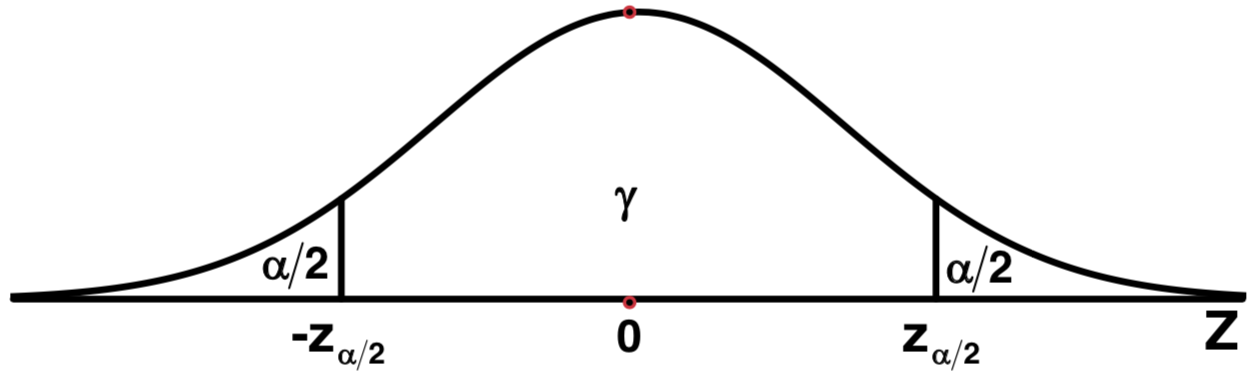
\includegraphics[width=6.5cm]{Graficos/fig1_CE}		}{  \caption*{}	}
	%
\end{floatrow}
\end{figure}
	
	\vspace{-3\baselineskip}
	%
	Cuando no se especifica el valor de \(\gamma\) y no se pide calcularlo, se supone que su valor es igual a \(0.95\).
\end{observ}


\begin{proposicion}
	Intervalo de confianza para la media \(\mu=\Esp[X]\), conocida \(\sigma^2=\Var[X]\); \(\bar{x}-B<\mu\bar{x}+B\), donde \(B=z_{\nicefrac{\alpha}{2}}\sqrt{\Var[\bar{X}]}\) y \(\Var[\bar{X}]=\dfrac{\sigma^2}{n}\).
\end{proposicion}
\begin{proof}
	Por el Teorema del Límite Central, si \(X\sim\Normal(\mu,\sigma^2)\) o \(n\) es suficientemente grande, \(\bar{X}\sim\Normal\left(\mu,\dfrac{\sigma^2}{n}\right)\), por lo que \(\Var[\bar{X}]=\dfrac{\sigma^2}{n}\), entonces \(Z=\nicefrac{\bar{X}-\mu}{\sigma}\sqrt{n}\) y \(P(-z_{\nicefrac{\alpha}{2}}<Z<z_{\nicefrac{\alpha}{2}})=\gamma\), lo cual es lo mismo que \(P\left(-z_{\nicefrac{\alpha}{2}}<\dfrac{\bar{X}-\mu}{\sigma}\sqrt{n}<z_{\nicefrac{\alpha}{2}}\right)=\gamma\), de donde \(P\left(\bar{X}-z_{\nicefrac{\alpha}{2}}\dfrac{\sigma}{\sqrt{n}}<\mu<\bar{X}+z_{\nicefrac{\alpha}{2}}\dfrac{\sigma}{\sqrt{n}}\right)=\gamma\). Por este resultado y utilizando la observación \eqref{obs-4.2}; \(B=z_{\nicefrac{\alpha}{2}}\dfrac{\sigma}{\sqrt{n}}\).  Como \(\Var[\bar{X}]=\dfrac{\sigma^2}{n}\), \(B\) se puede escribir como \(B=z_{\nicefrac{\alpha}{2}}\sqrt{\Var[\bar{X}]}\).
\end{proof}

\begin{observ}\label{obs-4.4}
	Por el resultado obtenido para \(B\): \(B=z_{\nicefrac{\alpha}{2}}\dfrac{\sigma}{\sqrt{n}}\)
	\begin{APAenumerate}
		\item \(B\) y \(n\) son inversamente proporcionales; por lo tanto, si se resuelve disminuir el límite para el error de estimación \(B\),  se debe incrementar el tamaño de la muestra \(n\).
		\item \(n=\dfrac{z_{\nicefrac{\alpha}{2}}^2\sigma^2}{B^2}\), por lo que \(z_{\nicefrac{\alpha}{2}}\) y \(n\) son directamente proporcionales. Si se resuelve aumentar el nivel de confianza \(\gamma\), se debe aumentar	 el valor de \(z_{\nicefrac{\alpha}{2}}\) con lo cual \(\gamma\) y \(n\) son directamente proporcionales; es decir, si se resuelve incrementar el valor de \(\gamma\), se debe incrementar el tamaño de la muestra.
	\end{APAenumerate}

Como para todo intervalo de confianza se aspira que sea pequeño el límite para el error de estimación y el nivel de confianza lo más grande posible, por los análisis realizados, el tamaño de la muestra debe ser suficientemente grande; lo que se opone a otras variables que intervienen en los procesos de muestreo tales como: costos, tiempo, recursos humanos, etc.

Por lo anterior, en la mayoría de estudios referentes a muestreo, uno de los aspectos fundamentales es el cálculo del tamaño de la muestra, para lo que se consideran a más del límite para el error de estimación y el nivel de confianza, otras variables como las mencionadas que no siempre es posible cuantificarlas
de manera más o menos precisa.
\end{observ}



%
%%%
%%%%% 	
%%%%%%%
\subsection{Muestreo aleatorio simple}

\neodefi{Sin considerar el tamaño de la población}

\neodefi{Para la media} 

Para estimar la media de una variable cuantitativa en una población a través de intervalos de confianza, existen dos posibilidades como consecuencia de la medida de variabilidad que se conozca:

\vspace{0.75\baselineskip}
	\textbf{Si se conoce la varianza \(\sigma^2\) (o la desviación estándar \(\sigma\)) de la variable en la población en estudio}\newline


Se utiliza lo desarrollado en la proposición \eqref{prop-4.2} \(\), \(\bar{x}-B<\mu<\bar{x}+B\), donde \(Bz_{\nicefrac{\alpha}{2}} 	\sqrt{\Var[\bar{X}]}\), \(\Var[\bar{X}]=\dfrac{\sigma^2}{n}\).

\begin{ejem}
	Un psicólogo desea estimar el tiempo medio de reacción de sus pacientes, para un estímulo especial, suponiendo que la desviación estándar de ese tiempo es igual a \(0.8\) segundos.
	\begin{APAenumerate}
		\item Con una muestra aleatoria de 73 pacientes obtuvo un promedio de \(4.1\) segundos. Calcule el intervalo de confianza para la media, al \(93\%\).
		\item Calcule el tamaño mínimo de la muestra para estimar la media poblacional si la longitud del intervalo de confianza es igual a \(0.32\) segundos y el nivel de confianza igual a \(0.96\).
	\end{APAenumerate}
\end{ejem}

\begin{proof}[Solución]\quad
	\begin{enumerate}
		\item \(n=73\); \(\bar{x}=42\); \(\sigma=0.8\); \(\gamma=0.93\)
		
		\(\bar{x}-B<\mu<\bar{x}+B\); \(B=z_{\nicefrac{\alpha}{2}}\sqrt{\Var[\bar{X}]}\); \(\Var[\bar{X}]=\dfrac{\sigma^2}{n}\); \(B=z_{\nicefrac{\alpha}{2}}\sqrt{\dfrac{\sigma^2}{n}}\); \(P(Z<z_{\nicefrac{\alpha}{2}})=0.965\); \(z_{\nicefrac{\alpha}{2}}=1.81\)
		
		\(B=1.81\sqrt{\dfrac{0.8^2}{73}}=1.69\); \(4.1-0.169<\mu<4.1+0.169\); \(3.931<\mu<4.269\)
		
		\vspace{1\baselineskip}
		\item \(\sigma=0.8\); \(L=0.32\); \(\gamma=0.96\)
		
		Para calcular el tamaño de la muestra: \(B=z_{\nicefrac{\alpha}{2}}\sqrt{\dfrac{\sigma^2}{n}}\), de donde \(n=\dfrac{z_{\nicefrac{\alpha}{2}}^2\sigma^2}{B^2}\)
		
		\(B=\dfrac{L}{2}=\dfrac{0.32}{2}=0.16\); \(P(Z<z_{\nicefrac{\alpha}{2}})=0.98\);
		
		\(z_{\nicefrac{\alpha}{2}}=2.05\); \(n=\dfrac{2.05^2 \times 0.8^2}{0.16^2}=105.0625\)
		
		El tamaño de toda muestra \(n\) es un número entero y \(B\) se define como el límite para el error de estimación, por lo que el resultado obtenido para \(n\) debe aproximarse.
		
		Si \(n=105\), \(B=z_{\nicefrac{\alpha}{2}}\sqrt{\dfrac{\sigma^2}{n}}=2.05\sqrt{\dfrac{0.8^2}{105}}=1.160047\)
		
		Si \(n=106\), \(B=z_{\nicefrac{\alpha}{2}}\sqrt{\dfrac{\sigma^2}{n}}=2.05\sqrt{\dfrac{0.8^2}{106}}=0.15929\)
		
		Por lo tanto, el tamaño mínimo de la muestra es igual a \(106\).			\qedhere
	\end{enumerate}
\end{proof}



\vspace{0.75\baselineskip}
	\textbf{Si se conoce la varianza \(s^2\) (o la desviación estándar \(s\)) de una muestra de la población en estudio (no se conoce \(\sigma^2\)).}\newline

\begin{proposicion}\label{prop-5.1}
	La variable \(T=\dfrac{\bar{X}-\mu}{S}\sqrt{n}\) tiene una distribución \(t\) de student con \(n-1\) grados de libertad.
\end{proposicion}


\begin{proposicion}\label{prop-5.2}
	El intervalo de confianza para la media \(\mu\) está dado por \(\bar{x}-B<\mu<\bar{x}+B\), con \(B=t_{\nicefrac{\alpha}{2},n-1} \sqrt{\Var[\bar{X}]}\); \(\Var[\bar{X}]=\dfrac{s^2}{n}\).
\end{proposicion}
\begin{proof}
	\(\bar{X}\) es estimador insesgado de \(\mu\), entonces \(P(\bar{X}-B<\mu<\bar{X}+B)=\gamma\) y el intervalo de confianza es igual a \(\bar{x}-B<\mu<\bar{x}+B\).
	
	Por la proposición \eqref{prop-5.1} y el comportamiento de la distribución \(t\) de student 
	\[
		P(-t_{\nicefrac{\alpha}{2},n-1}<T<t_{\nicefrac{\alpha}{2},n-1})= P\left(-t_{\nicefrac{\alpha}{2},n-1}<\dfrac{\bar{X}-\mu}{s}<t_{\nicefrac{\alpha}{2},n-1}\right)=\gamma,
	\]
	de donde  
	\[
		P\left(\bar{X}-t_{\nicefrac{\alpha}{2},n-1}\dfrac{s}{\sqrt{n}}<\mu<\bar{X}+t_{\nicefrac{\alpha}{2},n-1}\dfrac{s}{\sqrt{n}}\right)=\gamma. 
	\]	
	Por lo tanto: \(B=t_{\nicefrac{\alpha}{2},n-1}\dfrac{s}{\sqrt{n}}\).
	
	\(s^2\) estima a \(\sigma^2\), \(\Var[\bar{X}]=\dfrac{s^2}{n}\) estima a \(\Var[\bar{X}]=\dfrac{\sigma^2}{n}\), con lo cual \(B=t_{\nicefrac{\alpha}{2},n-1}\sqrt{\Var[\bar{X}]}\); \(\Var[\bar{X}]=\dfrac{s^2}{n}\).
\end{proof}


\begin{observ}\quad
	\begin{APAenumerate}
		\item Los valores de la distribución \(t\) de student son similares a los de la distribución normal estándar, cuando \(n\) toma valores altos.
		\item Para calcular \(t_{\nicefrac{\alpha}{2},n-1}\), se utiliza la relación \(P(T>t_{\nicefrac{\alpha}{2},n-1})=\dfrac{\alpha}{2}\), con \(\gamma+\alpha=1\).
	\end{APAenumerate}
\end{observ}


\begin{ejem}
	En un estudio de mercado sobre la cantidad mensual utilizada para adquirir productos de aseo personal.
	\begin{enumerate}
		\item Se tomó una muestra de 54 familias, obteniéndose que en promedio utilizaban \(67.2\) dólares mensuales y la desviación estándar era igual a \(39.5\) dólares. Calcule el intervalo de confianza para la cantidad mensual media familiar empleada en productos de aseo personal, al \(90\%\).
		\item Calcule el tamaño mínimo muestral necesario para calcular el intervalo de confianza para la cantidad mensual media que utiliza la población en estudio para adquirir productos de aseo, si el límite para el error de estimación es igual a \(7.9\) dólares y el nivel de confianza es igual a \(0.94\).
	\end{enumerate}
\end{ejem}
\begin{proof}[Solución]\quad
	\begin{APAenumerate}
		\item \(n=54\); \(\bar{x}=62.7\); \(s=39.5\), \(\gamma=0.9\)
		
		\(\bar{x}-B<\mu<\bar{x}+B\); \(B=t_{\nicefrac{\alpha}{2},n-1}\sqrt{\Var[\bar{X}]}\); \(\Var[\bar{X}]=\dfrac{s^2}{n}\), entonces \(B=t_{\nicefrac{\alpha}{2},n-1}\sqrt{\dfrac{s^2}{n}}\)
		
		\(P(T_{53}>t_{\nicefrac{\alpha}{2},n-1})=0.05\); \(t_{\nicefrac{\alpha}{2},n-1}=1.673\) (aproximadamente \(53\) a \(55\) y utilizando la tabla 2 de este documento)
		
		\(B=1.673\sqrt{\dfrac{39.5^2}{54}}=8.842\), entonces \(67.2-8.842<\mu<67.2+8.842\); \(58.358<\mu<76.042\) 
		
		\vspace{1\baselineskip}
		\item \(s=39.5\); \(B=7.9\); \(\gamma=0.94\)
		
		De \(B=t_{\nicefrac{\alpha}{2},n-1}\sqrt{\dfrac{s^2}{n}}\); \(n=\dfrac{t_{\nicefrac{\alpha}{2},n-1}^2s^2}{B^2}\).
		
		Como no se conoce el valor de \(n\) (lo que se solicita), no es posible obtener \(t_{\nicefrac{\alpha}{2},n-1}\), por lo que aproximamos su valor con el de \(z_{\nicefrac{\alpha}{2}}\); \(P(Z<z_{\nicefrac{\alpha}{2}})=0.97\); \(z_{\nicefrac{\alpha}{2}}=1.88\)
		
		\(n=\dfrac{1.88^2*39.5^2}{7.9^2}=88.26\); \(n =89\)
		
		Para calcular \(n\) se utilizó la distribución normal en lugar de  la distribución de student, por lo que es necesario realizar un ajuste, comenzando con el valor calculado para \(n\), hasta obtener el mínimo valor que garantice que el valor de \(B\) no supere al determinado (\(7.9\)).
		
		Ajuste
		\[
		P(T_{n-1}>t_{\nicefrac{\alpha}{2},n-1})=0.03
		\]
		\vspace{-1\baselineskip}
		
	\begin{table}[H]
	\fontsize{7.25}{11}\selectfont
	\centering
	\begin{tabular}{l  c cc cc} \thickline
		\(n\) & \(n-1\) 	&	\(t_{\nicefrac{\alpha}{2},n-1}\)	&  \(B=t_{\nicefrac{\alpha}{2},n-1}\sqrt{\dfrac{s^2}{n}}\) 
		\vspace{0.5em}
	 		\\     \hline
		89    & 88(90)  	& 1.9048                           & \(B=1.9048\sqrt{\dfrac{38.9^2}{89}}\approx 7.975\)             \\
		90    & 89(90)  	& 1.9048                           & \(B=1.9048\sqrt{\dfrac{39.5^2}{90}}\approx 7.931\)             \\
		91    & 90      	& 1.9048                           & \(B=1.9048\sqrt{\dfrac{39.5^2}{91}}\approx 7.887\)                                                                          
	\end{tabular}
	\end{table}
		
	El tamaño mínimo de la muestra es \(91\).			\qedhere
	\end{APAenumerate}
\end{proof}



\neodefi{Para la proporción}

Para la proporción, \(X\): <<Número de éxitos en los \(n\) procesos de Bernoulli>>, donde \(P(E)=p\) y \(P(F)=q=1-p\) constantes para los \(n\) procesos \(X_1.X_2.\ldots,X_n\) aleatorios e independientes, con 
\[
	X_i=\begin{cases} 1 & E,\\ 0 & F;\end{cases}
	\qquad
	P(X_i=1)=P(E)=p;
	\qquad
	P(X_i=0)=P(F)=q;
\]
y \(\Esp[X_i]=p\), \(\Var[X_i]=pq\), para todo \(i \in \{1.\ldots,n\}\); con lo cual se puede escribir: \( X=\displaystyle\sum_{i=1}^{n}X_i\), entonces \(P=\dfrac{X}{n}=\dfrac{1}{n}\dsum_{i=1}^{n}X_i=\bar{X}\).

\begin{proposicion}
	El intervalo de confianza para la proporción \(p\), conocida \(p\) está dado por \(\hat{p}-B<p<\hat{p}+B\), donde: \(B=z_{\nicefrac{\alpha}{2}}\sqrt{\Var[\hat{p}]}\); \(\Var[\hat{p}]=\dfrac{pq}{n}\).
\end{proposicion}
\begin{proof}
	Por la proposición \eqref{prop-4.1}, \(P=\dfrac{X}{n}=\dfrac{1}{n}\displaystyle\sum_{i=1}^{n}X_i=\bar{X}\) es un estimador insesgado de \(p\). Por la definición \eqref{def-4.4} \(P\big(\left|\hat{P}-p\right|<B\big)=\gamma\), lo que es equivalente a  \(P(\hat{P}-B<p<\hat{P}-p)=\gamma\) y el intervalo de confianza para  \(p\) es \(\hat{p}-B<p<\hat{p}+B\).
	
	Como \(P=\bar{X}\), utilizando el Teorema del Límite Central, \(P=\bar{X}\sim\Normal\big(\Esp[\hat{P}],\Var[\hat{P}]\big)\) asintóticamente (\(n\) suficientemente grande).
	
	Por los resultados obtenidos en la proposición \eqref{prop-4.1} \(\Esp[\hat{P}]=p\) y \(\Var[\hat{P}]=\dfrac{pq}{n}\); por lo tanto, \(P\sim\Normal\left(p,\dfrac{pq}{n}\right)\). Entonces \(Z=\dfrac{\bar{X}-\mu}{\sigma}\sqrt{n}\) y \(P(-z_{\nicefrac{\alpha}{2}}<Z<z_{\nicefrac{\alpha}{2}})=\gamma\)
	
	\begin{figure}[H]
\hspace{-3.5em}
\begin{floatrow}
	\fontsize{8}{11}\selectfont
	\captionsetup{justification=centering, labelfont=footnotesize, font=footnotesize}
	%	Tabla
	\capbtabbox{%
	$
	P( Z<z_{\nicefrac{\alpha}{2}} )=
	\begin{cases}
		1-\nicefrac{\alpha}{2} \\
		\nicefrac{\alpha}{2}+\gamma \vspace{2.5\baselineskip} \\
		\dfrac{1+\gamma}{2}
	\end{cases}
	$
	\vspace{2.1em}
	}{	  \caption*{}%
	}
	%	Figura
	\ffigbox{	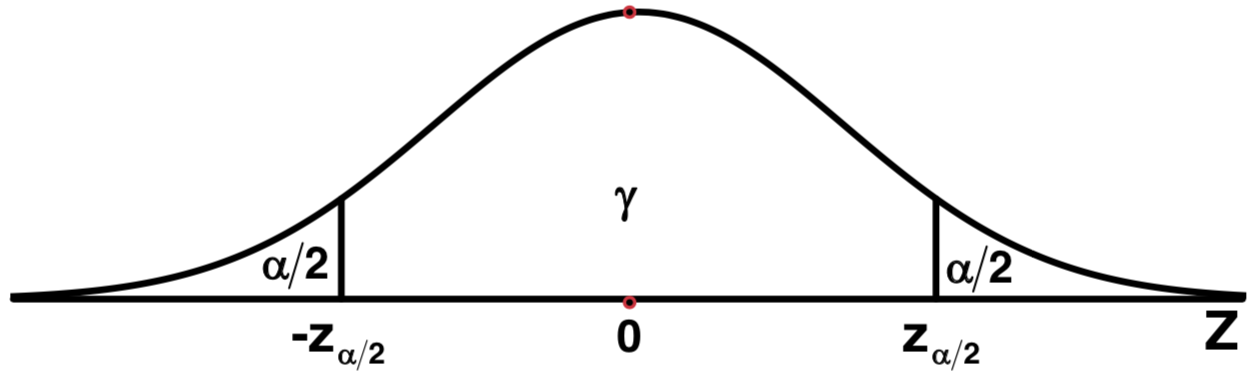
\includegraphics[width=6.5cm]{Graficos/fig1_CE}		}{  \caption*{}	}
	%
\end{floatrow}
\end{figure}
	
	\vspace{-3\baselineskip}
	\(P\left(-z_{\nicefrac{\alpha}{2}}<\dfrac{\bar{X}-p}{pq}\sqrt{n}<z_{\nicefrac{\alpha}{2}}\right)=\gamma\), de donde \(P\left(\bar{X}-z_{\nicefrac{\alpha}{2}}\dfrac{p1}{\sqrt{n}}<p<\bar{X}+z_{\nicefrac{\alpha}{2}}\dfrac{pq}{\sqrt{n}}\right)=\gamma\), con lo cual \(B=z_{\nicefrac{\alpha}{2}}\dfrac{pq}{n}\) y como \(\Var[\hat{P}]=\dfrac{pq}{n}\), \(B\) se puede escribir como \(B=z_{\nicefrac{\alpha}{2}}\dfrac{pq}{\sqrt{n}}\).
\end{proof}

\begin{ejem}
	El auditor de una empresa está interesado en conocer la proporción de comprobantes que podrían 	estar archivados incorrectamente. Se sabe que en empresas similares, el \(8\%\) de los comprobantes se archivan incorrectamente
	\begin{APAenumerate}
		\item Calcule el intervalo de confianza para la proporción de comprobantes que podrían estar mal archivados, si se toma una muestra de tamaño \(172\).
		\item Si se fija la longitud del intervalo de confianza en \(0.066\) y el nivel de confianza en \(0.93\), calcule el tamaño de muestra mínimo necesario para hacer el estudio.
	\end{APAenumerate}
\end{ejem}
\begin{proof}[Solución]\quad
	\begin{APAenumerate}
		\item \(p=0.08\); \(n=172\); \(\gamma=0.95\)
		
		\(B=z_{\nicefrac{\alpha}{2}}\sqrt{\Var[\hat{P}]}\), donde \(\Var[\hat{P}]=\dfrac{pq}{n}\); \(B=z_{\nicefrac{\alpha}{2}}\sqrt{\dfrac{pq}{n}}\); \(P(Z<z_{\nicefrac{\alpha}{2}})=0.975\); \(z_{\nicefrac{\alpha}{2}}=1.96\).
		
		Entonces  \(B=1.96\sqrt{\dfrac{0.08 \times 0.92}{172}}=0.0405\).
		
		Como se conoce el valor de \(p\), el intervalo de confianza es igual a 
		\[0.08-0.0405<p<0.08+0.0405 ; \qquad 0.0395<p<0.1205.\]
		
		\vspace{1\baselineskip}
		\item \(p=0.08\); \(\gamma=0.93\); \(L=0.066\); \(B=0.033\); \(P(Z<z_{\nicefrac{\alpha}{2}})=0.965\); \(z_{\nicefrac{\alpha}{2}}=1.81\)
		
		\(B=z_{\nicefrac{\alpha}{2}}\sqrt{\dfrac{pq}{n}}\), de donde \(n=\dfrac{z_{\nicefrac{\alpha}{2}}^2*pq}{B^2}\); \(n=\dfrac{1.81^2 \times 0.08 \times 0.92}{0.033^2}=221.415\). El tamaño mínimo de la muestra es \(222\).		\qedhere
	\end{APAenumerate}
\end{proof}


\begin{proposicion}\label{prop-5.4}
	El intervalo de confianza para la proporción \(p\), conocida \(\hat{p}\) está dado por \(\hat{p}-B<p<\hat{p}+B\), donde \(B=z_{\nicefrac{\alpha}{2}}\sqrt{\Var[\hat{P}]}\); \(\Var[\hat{P}]=\dfrac{pq}{n}\).
\end{proposicion}
\begin{proof}
	Por la proposición \eqref{prop-4.1}, \(P=\dfrac{X}{n}=\dfrac{1}{n}\displaystyle\sum_{i=1}^{n}X_i=\bar{X}\) es un estimador insesgado de \(p\). Por lo tanto \(P(\hat{P}-B<p<\hat{P}-B)=\gamma\) y el intervalo de confianza para \(p\) es \(\hat{p}-B<p<\hat{p}+B\).
	
	\(\hat{p}\) estima a \(p\); \(\Var[\hat{P}]\dfrac{pq}{n}\) estima a \(\Var[P]=\dfrac{pq}{n}\), con lo cual por lo tanto \(\hat{p}-B<p<\hat{p}+B\) es el intervalo de confianza para \(p\), con \(B=z_{\nicefrac{\alpha}{2}}\sqrt{\Var[\hat{P}]}\); \(\Var[\hat{P}]=\dfrac{pq}{n}\).
\end{proof}


\begin{observ}
	Si nada se conoce como \(p\), se considera a \(p=q=0.5\), ya que, como primera aproximación, con esos valores se obtiene el mayor valor posible para \(B=z_{\nicefrac{\alpha}{2}}\sqrt{\dfrac{pq}{n}}\).
\end{observ}

\begin{ejem}
	Con una muestra piloto de \(764\) votantes respecto a que la Asamblea Nacional elija a los miembros de la Corte Suprema de Justicia, el \(20\%\) respondió estar de acuerdo.
	\begin{APAenumerate}
		\item Calcule el intervalo de confianza al \(95\%\) para la proporción de votantes que están de acuerdo con ese planteamiento.
		\item Se ha resuelto que se realice el estudio definitivo con el límite para el error de estimación igual a \(0.02\) y el nivel de confianza igual a \(0.97\). Calcule el tamaño mínimo de muestra para realizar el estudio.
	\end{APAenumerate}
\end{ejem}
\begin{proof}[Solución]\quad
	\begin{APAenumerate}
		\item \(n=764\); \(p=0.2\); \(\gamma=0.95\); \(P(Z<z_{\nicefrac{\alpha}{2}})=0.975\); \(z_{\nicefrac{\alpha}{2}}=1.96\)
		
		\(\hat{p}-B<p<\hat{p}+B\), \(B=z_{\nicefrac{\alpha}{2}}\sqrt{\Var[\hat{P}]}\); \(\Var[\hat{P}]=\dfrac{pq}{n}\); \(B=z_{\nicefrac{\alpha}{2}}\sqrt{\dfrac{pq}{n}}\), entonces 
		
		\(B=1.96\sqrt{\dfrac{0.2 \times 0.8}{764}}=0.0283641\); \(0.1-0.0283541<p<0.2+0.0283641\); \(0.1716359<p<0.02283641\).
		
		\vspace{1\baselineskip}
		\item \(B=0.025\); \(p=0.2\); \(\gamma=0.96\); \(P(Z<z_{\nicefrac{\alpha}{2}})=0.98\); \(z_{\nicefrac{\alpha}{2}}=2.05\); \(B=z_{\nicefrac{\alpha}{2}}\sqrt{\dfrac{\hat{p}{\hat{q}}}{n}}\); \(n=\dfrac{z_{\nicefrac{\alpha}{2}}^2\hat{p}\hat{q}}{B^2}\)
		\(n=\dfrac{2.05^2 \times 0.2 \times 0.8}{0.025^2}=1075.84\); \(n=1076\).		\qedhere
	\end{APAenumerate}
\end{proof}

%
%
%
\newpage
\neodefi{Muestreo aleatorio simple considerando el tamaño de la población}


\begin{proposicion}
	Supóngase una población de \(N\) elementos que tienen igual probabilidad de ser incluidos en cualquier muestra extraída al azar; \(y_1.y_2.\ldots,y_n\) representan los valores asignables a cada uno de los elementos de la población al aplicársele una variable aleatoria \(X\); \(\Esp[X]=\mu\); \(\Var[X]=\sigma^2\); \(X_1.X_2.\ldots,X_n\)una muestra de variables aleatorias idénticamente distribuidas (que se obtienen al aplicar \(n\) veces \(X\) en la población) con \(\Esp[X_i]=\mu\); \(\Var[X_i]=\sigma^2\); \(\bar{X}=\dfrac{1}{n}\displaystyle\sum_{i=1}^{n}X_i\); \(S^2=\dfrac{1}{n-1}\displaystyle\sum_{i=1}^{n}(X_i-\bar{X})^2\). Entonces:
	\begin{APAenumerate}
		\item \(\Esp[\bar{X}]=\Esp[X]=\mu\) (\(\bar{X}\) es un estimador insesgado de \(\Esp[X]\)),
		\item \(\cov(X_i,X_j)=-\dfrac{\sigma^2}{N-1}\),
		\item \(\Var[\bar{X}]=\dfrac{s^2}{n}\left(\dfrac{N-n}{N-1}\right)\),
		\item \(\Esp[S^2]=\dfrac{\sigma^2N}{N-1}\),
		\item Si \(\Var[\bar{X}]=\dfrac{s^2}{n}\left(\dfrac{N-n}{N}\right)\), entonces  \(\Esp\big[\Var[\bar{X}]\big]=\Var[\bar{X}]\)
		(\(\Var[\bar{X}]\) es un estimador insesgado de \(\Var[X]\)).
	\end{APAenumerate}
\end{proposicion}


\neodefi{Para la media} 

El intervalo de confianza para la media: \(\bar{x}-B<\mu<\bar{x}+B\).

\vspace{0.75\baselineskip}
	\textbf{Si se conoce la varianza \(\sigma^2\)(o la desviación estándar \(\sigma\)) de la variable en la población en estudio}
	\[
		B=z_{\nicefrac{\alpha}{2}}\sqrt{\Var[\bar{X}]}, \qquad \Var[\bar{X}]=\dfrac{\sigma^2}{n}\left(\dfrac{N-n}{N-1}\right)
	\]
	

\begin{ejem}
	En la fabricación de \(1462\) soportes de caucho se ha resuelto trabajar con las siguientes condiciones: el intervalo de confianza para la media de dureza igual a \([158 ; 165] \) la varianza del proceso igual a \(169\); el nivel de confianza del intervalo igual a \(0.92\). Calcule el tamaño mínimo de la muestra que cumple con las condiciones planteadas.
\end{ejem}
\begin{proof}[Solución]\qquad

		\(N=1462\); \([158;165]\); \(\sigma^2=169\); \(\gamma=0.92\); \(P(Z<z_{\nicefrac{\alpha}{2}})=0.96\); \(z_{\nicefrac{\alpha}{2}}=1.75\)
		
		\(B=z_{\nicefrac{\alpha}{2}}\sqrt{\Var[\bar{X}]}\); \(\Var[\bar{X}]=\dfrac{\sigma^2}{n}\left(\dfrac{N-n}{N-1}\right)\); \(B=z_{\nicefrac{\alpha}{2}}\sqrt{\dfrac{\sigma^2(N-n)}{n(N-1)}}\)
		
		\(n=\dfrac{z_{\nicefrac{\alpha}{2}}^2\sigma^2 N}{B^2(N-1)+z_{\nicefrac{\alpha}{2}}^2\sigma^2}=\dfrac{1.75^2 \times 169 \times 1462}{3.5^2 \times 1461+1.75^2 \times 169}=41.0906\ldots\); \(n=42\)
\end{proof}


\vspace{0.75\baselineskip}
	\textbf{Si se conoce la varianza \(s^2\) (o la desviación estándar \(s\)) de una muestra de la población en estudio (no se conoce \(\sigma^2\)) }
	\[
		B=t_{\nicefrac{\alpha}{2},n-1}\sqrt{\Var[\bar{X}]}; \qquad
		\Var[\bar{X}]=\dfrac{s^2}{n}\left(\dfrac{N-n}{N}\right)
	\]
	

\begin{ejem}
	Para producir \(587\) piezas se ha resuelto realizar una prueba con \(16\), respecto al peso (en gramos). La muestra piloto obtenida es:
	\[\begin{Bmatrix}
	97.9 & 88.0 & 94.6 & 97.0 & 98.1 & 80.1 & 79.9 & 87.1 \\
	 88.0 & 93.4 & 84.4 & 79.0 & 87.9 & 80.6 & 94.2 & 86.0
	\end{Bmatrix}\]

\begin{APAenumerate}
	\item Calcule el intervalo de confianza para la media de producción al \(93\%\). 
	\item Para el estudio muestral definitivo se ha resuelto fijar el límite para el error de estimación igual a \(2.4\) gramos y el nivel de confianza igual a \(0.96\). Calcule el tamaño mínimo de muestra que cumpla lo establecido.
\end{APAenumerate}
\end{ejem}
\begin{proof}[Solución]\quad
	\begin{APAenumerate}
		\item \(N=587\); \(n=16\); \(\gamma=0.93\); \(\bar{x}=88.5125\); \(s=6.681\ldots\); \(P(T_{15}>t_{\nicefrac{\alpha}{2},n-1})=0.035\); \(t_{\nicefrac{\alpha}{2},n-1}=1.9509\)
		
		\(\bar{x}-B<\mu<\bar{x}+B\); \(B=t_{\nicefrac{\alpha}{2},n-1}\sqrt{\Var[\bar{X}]}\); \(\Var[\bar{X}]=\dfrac{s^2}{n}\left(\dfrac{N-n}{N}\right)\);
		
		\(B=t_{\nicefrac{\alpha}{2},n-1}\sqrt{\dfrac{s^2(N-n)}{Nn}}=1.9509\sqrt{\dfrac{{6.681\ldots}^2(587-1)}{16 \times 587}}=3.21377\ldots\)
		
		\(88.5125-3.21377\ldots<\mu<88.5125+3.21377\ldots\); \(85.2987\ldots<\mu<91.72627\ldots\)
		
		\vspace{1\baselineskip}
		\item \(N=5887\); \(B=2.6\); \(\gamma=0.96\); \(s=6.681005...\);
		 
		\(B=t_{\nicefrac{\alpha}{2},n-1}\sqrt{\dfrac{s^2(N-n)}{Nn}}\); \(n=\dfrac{t_{\nicefrac{\alpha}{2},n-1}^2s^2N}{B^2N+t_{\nicefrac{\alpha}{2},n-1}^2s^2}\);
		
		Como no se conoce el valor de \(n\) (lo que se solicita), no es posible obtener \(t_{\nicefrac{\alpha}{2},n-1}\), por lo que 	aproximamos su valor con el de \(z_{\nicefrac{\alpha}{2}}\); \(P(Z<z_{\nicefrac{\alpha}{2}})=0.98\); \(z_{\nicefrac{\alpha}{2}}=2.05\)
		
		\(n=\dfrac{2.05^2 \times 6.681\ldots^2 \times 587}{2.6^2 \times 587+2.05^2 \times 6.681\ldots^2}=26.49\ldots\); \(n=27\)
		
		Para calcular \(n\) se utilizó la distribución normal en lugar de la distribución de student, por lo que es necesario realizar un ajuste, comenzando con el valor calculado para n, hasta obtener el mínimo valor que garantice que el valor de \(B\) no supere al determinado (\(2.6\)).
		
		Ajuste \[P(T_{n-1}>t_{\nicefrac{\alpha}{2},n-1})=0.02\]
		
		
	\vspace{-1\baselineskip}	
	\begin{table}[H]
	\fontsize{7.25}{11}\selectfont
	\centering
	\begin{tabular}{l  c cc cc} \thickline
		\(n\) & \(n-1\) 	&	\(t_{\nicefrac{\alpha}{2},n-1}\)	&  \(B=t_{\nicefrac{\alpha}{2},n-1}\sqrt{\dfrac{s^2(N-n)}{nN}} \) 
		\vspace{0.5em}
	 		\\     \hline
		27    & 26      & 2.162                            & 2.7151\ldots                                                  \\
		28    & 27      & 2.1578                           & 2.6586\ldots                                                  \\
		29    & 28      & 2.1539                           & 2.6053\ldots                                                  \\
		30    & 29      & 2.1503                           & 2.5549\ldots  
	\end{tabular}
	\end{table}

	
	El tamaño mínimo de la muestra es \(30\).				\qedhere
	\end{APAenumerate}
\end{proof}


\newpage

\neodefi{Para el total}

\begin{proposicion}\label{prop-5.6}\quad
	\begin{APAenumerate}
		\item \(\hat{T}=N\hat{X}\) es un estimador insesgado para el total \(T=N\mu\)
		\item Si se conoce la varianza \(\sigma^2\)(o la desviación estándar \(\sigma\)) de la variable en la población en estudio, el intervalo de confianza para el total está dado por \(\hat{t}-B<T<\hat{t}+B\), donde \(\hat{t}=N\bar{x}\); \(B=z_{\nicefrac{\alpha}{2}}\sqrt{\Var[\bar{T}]}\); \(\Var[\hat{T}]=N^2\Var[\bar{X}]\).
		\item Si se conoce la varianza \(s^2\) (o la desviación estándar \(s\)) de una muestra de la población en estudio (no se conoce \(\sigma^2\)), el intervalo de confianza total está dado por \(\hat{t}-B<T<\hat{t}+B\), donde \(\hat{t}=N\bar{x}\); \(B=t_{\nicefrac{\alpha}{2},n-1}\sqrt{\Var[\hat{T}]}\); \(\hat{\Var}[\hat{T}]=N^2\Var[\bar{X}]\).
	\end{APAenumerate}
\end{proposicion}
\begin{proof}\quad
	\begin{APAenumerate}
		\item El total \(T\) está dado por \(T=N\mu\). Como \(\bar{X}\) es un estimador insesgado de \(\mu\), \(\hat{T}=N\bar{x}\) es un estimador insesgado de \(T\), ya que \(\Esp[\hat{T}]=\Esp[N\bar{X}]=N\Esp[\bar{X}]=N\mu=T\).
		
		\vspace{1\baselineskip}
		\item El intervalo de confianza para \(\mu\) está dado por: \(\bar{x}-B<\mu<\bar{x}+B\); con \(B=z_{\nicefrac{\alpha}{2}}\sqrt{\Var[\bar{X}]}\)
		
		\(N\bar{x}-BN<N\mu<N\bar{x}+NB\); \(\hat{t}=N\bar{x}\); \(T=N\mu\)
		
		\(NB=Nz_{\nicefrac{\alpha}{2}}\sqrt{\Var[\bar{X}]}=z_{\nicefrac{\alpha}{2}}\sqrt{N^2\Var[\bar{X}]}=z_{\nicefrac{\alpha}{2}}\sqrt{\Var[\hat{T}]}\); luego \(\hat{t}-B<T<\hat{t}+B\) con \(B=z_{\nicefrac{\alpha}{2}}\sqrt{\Var[\hat{T}]}\); \(\Var[\hat{T}]=N^2\Var[\bar{X}]\).
		
		\vspace{1\baselineskip}
		\item El intervalo de confianza para \(\mu\) está dado por: \(\bar{x}-B<\mu<\bar{x}+B\); con \(B=t_{\nicefrac{\alpha}{2},n-1}\sqrt{\Var[\bar{X}]}\);
		
		\(N\bar{x}-NB<N\mu<N\bar{x}+NB\); \(\hat{t}=N\bar{x}\); \(T=N\mu\)
		
		\(NB=Nt_{\nicefrac{\alpha}{2},n-1}\sqrt{\Var[\bar{X}]}=t_{\nicefrac{\alpha}{2},n-1}\sqrt{N^2\Var[\bar{X}]}=t_{\nicefrac{\alpha}{2},n-1}\sqrt{\Var[\hat{T}]}\); luego \(\hat{t}-B<T<\hat{t}+B\), con \(B=t_{\nicefrac{\alpha}{2},n-1}\sqrt{\Var\hat{T}}\).									\qedhere
	\end{APAenumerate}
\end{proof}


\begin{ejem}\label{ejem-5.7}
	En el supermercado se está realizando un estudio sobre los ingresos anuales.
	\begin{APAenumerate}
		\item Con la muestra aleatoria piloto de los ingresos diarios (en miles de dólares) obtenida, calcule el intervalo de confianza para el total de los 365 días del año.
		\[\setcounter{MaxMatrixCols}{20}
		\begin{Bmatrix}
	4.66 & 3.85 & 3.97 & 5.02 & 4.14 & 4.24 & 3.42 & 4.22& 3.63 & 4.99  \\
	5.57 & 4.70 & 5.44 & 4.70 & 5.02 & 4.38 & 4.63 & 5.18 & 3.81 & 4.53 \\
	4.84 & 4.58 & 5.50 & 4.24 & 4.02 & 4.82 & 5.69 & 4.38 & 5.00 & 4.08
	\end{Bmatrix}\]

\item Para realizar el estudio definitivo se ha determinado que el límite para el error de estimación para el total sea igual a 7000 dólares y el nivel de confianza igual a \(0.97\). Calcule el tamaño mínimo de muestra que cumple lo dispuesto.
	\end{APAenumerate}
\end{ejem}
\begin{proof}[Solución]\quad
	\begin{APAenumerate}
		\item \(N=365\); \(n=30\); como no hay información sobre el nivel de confianza se supone que \(\gamma=0.95\); \(\bar{x}=4.575\); \(s=0.587177\ldots\); \(P(T_{29}<t_{\nicefrac{\alpha}{2},n-1})=0.025\); 
		
		\(t_{\nicefrac{\alpha}{2},n-1}=2.0452\) \(\hat{t}-B<T<\hat{t}+B\); \(\hat{t}=N\bar{x}=365 \times 4.575=1669.875\)
		
		\(B=t_{\nicefrac{\alpha}{2},n-1}\sqrt{\Var[\hat{T}]}\); \(\Var[\hat{T}]=N^2\Var[\bar{X}]=\dfrac{N^2s^2(N-n)}{nN}=\dfrac{Ns^2(N-n)}{n}\), entonces
		
		\(B=t_{\nicefrac{\alpha}{2},n-1}\sqrt{\Var[\hat{T}]}=t_{\nicefrac{\alpha}{2},n-1}\sqrt{\dfrac{Ns^2(N-n)}{n}}=\dfrac{365 \times 0.587177\ldots^2(365-30)}{30}=76.66788\ldots\);
		
		\(1666.875-76.66788\ldots<T<1666.875+76.6788\ldots\)
		
		\(1593.2071\ldots<T<1746.5428\ldots\)
		
		\vspace{1\baselineskip}
		\item \(N=365\); \(B=70\); \(\gamma=0.97\); \(s=	0.587177\ldots\);
		
		\(B=t_{\nicefrac{\alpha}{2},n-1}\sqrt{\dfrac{Ns^2(N-n)}{n}}\); \(n=\dfrac{t_{\nicefrac{\alpha}{2},n-1}^2N^2s^2}{B^2+t_{\nicefrac{\alpha}{2},n-1}^2Ns^2}\);
		
		Como no se conoce el valor de \(n\) (lo que se solicita), no es posible obtener \(t_{\nicefrac{\alpha}{2},n-1}\)por lo que aproximaremos su valor con el de \(z_{\nicefrac{\alpha}{2}}\); \(P(Z<z_{\nicefrac{\alpha}{2}})=0.985\); \(z_{\nicefrac{\alpha}{2}}=2.17\)
		
		\(n=\dfrac{2.17^2 \times 365 \times 0.587177\ldots^2}{70^2+2.17^2 \times 365 \times 6.681\ldots^2}=39.379\); \(n=40\)
		
		Para calcular \(n\) se utilizó la distribución normal en lugar de la distribución  de student, por lo que es necesario realizar un ajuste, comenzando con el valor calculado para \(n\), hasta obtener el mínimo valor que garantice que el valor de \(B\) no supere determinado (\(70\)).
		
		Ajuste \[P(T_{n-1}>t_{\nicefrac{\alpha}{2},n-1})=0.015\]

	\vspace{-1\baselineskip}	
	\begin{table}[H]
	\fontsize{7.25}{11}\selectfont
	\centering
	\begin{tabular}{l  c cc cc} \thickline
		\(n\) & \(n-1\) 	&	\(t_{\nicefrac{\alpha}{2},n-1}\)	&  \(B=t_{\nicefrac{\alpha}{2},n-1}\sqrt{\dfrac{s^2(N-n)}{nN}} \) 
		\vspace{0.5em}
	 		\\     \hline
		40    & 39(40)  & 2.2503                           & 71.956                                                        \\
		41    & 40      & 2.2503                           & 70.963                                                        \\
		42    & 41(40)  & 2.2503                           & 70.0056                                                       \\
		43    & 42(40)  & 2.2503                           & 69.079  
	\end{tabular}
	\end{table}

	
	El tamaño mínimo de la muestra es \(43\).			\qedhere
	\end{APAenumerate}
\end{proof}


\neodefi{Para la proporción}


\begin{proposicion}\label{prop-5.7}
	Dados \(n\) procesos de Bernoulli con \(P(E)=p\) y \(P(F)=q=1-p\) constantes para los \(n\) procesos; \(X_1.X_2.\ldots,X_n\) variables aleatorias con
	\[
	X_i=\begin{cases} 1 & E,\\ 0 & F;\end{cases}
	\qquad
	P(X_i=1)=P(E)=p;
	\qquad
	P(X_i=0)=P(F)=q;
\]
y \(\Esp[X_i]=p\), \(\Var[X_i]=pq\), para todo \(i \in \{1.\ldots,n\}\); \(X\): <<Número de éxitos en los \(n\) procesos>>; \(p=\dfrac{x}{n}\). Entonces
	\begin{APAenumerate}
		\item \(\Var[\hat{P}]=\dfrac{pq}{n}\left(\dfrac{N-n}{N-1}\right)\),
		\item \(s^2=\dfrac{n\hat{p}\hat{q}}{n-1}\),
		\item \(\hat{\Var}[\hat{P}]=\dfrac{\hat{p}\hat{q}}{n-1}\left(\dfrac{N-1}{N}\right)\).
	\end{APAenumerate}
\end{proposicion}

\begin{observ}
	Por la proposición \eqref{prop-5.7}: El intervalo de confianza para la proporción\(p\), conocida \(p\), está dado por \(\hat{p}-B<p<\hat{p}+B\), donde \(B=z_{\nicefrac{\alpha}{2}}\sqrt{\Var[\hat{P}]}\); \(\Var[\hat{P}]=\dfrac{pq}{n}\left(\dfrac{N-n}{N-1}\right)\).
	
	El intervalo de confianza para la proporción \(p\), conocida \(\hat{p}\), está dado \(\hat{p}-B<p<\hat{p}+B\), donde \(B=z_{\nicefrac{\alpha}{2}}\sqrt{\hat{\Var}[\hat{P}]}\); \(\hat{\Var}[\hat{P}]=\dfrac{\hat{p}\hat{q}}{n-1}\left(\dfrac{N-n}{N}\right)\).
	
	Si nada se conoce sobre \(p\), se cnsidera que \(p=q=0.5\) ya que, como primera aproximación, con esos valores se obtiene el mayor valor posible para \(B=z_{\nicefrac{\alpha}{2}}\sqrt{\Var[\hat{P}]}\).
\end{observ}



\begin{ejem}
	Se ha resuelto realizar un estudio sobre el uso de compras por internet en una población de 3734 familias.
	\begin{APAenumerate}
		\item Con una muestra piloto de 250 familias se obtuvo que 162 realizaban compras por ese sistema. Calcule el intervalo de confianza para la proporción de familias que compran por internet, al \(91\%\).
		\item Con base a lo obtenido en la solución de la primera pregunta, calcule el mínimo y el máximo número de familias que se esperaría realicen compras por internet.  
		\item Si se aspira a realizar el estudio definitivo al \(93\%\) con el límite para el error de estimación igual a \(0.04\), calcule el tamaño mínimo de muestra.
	\end{APAenumerate}
\end{ejem}
\begin{proof}[Solución]\quad
	\begin{APAenumerate}
		\item \(N=3734\); \(n=250\); \(x=162\); \(\gamma=0.91\)
		
		\(\hat{p}-B<p<\hat{p}+B\); \(B=z_{\nicefrac{\alpha}{2}}\sqrt{\hat{\Var}[\hat{P}]}\); \(\hat{\Var}[\hat{P}]=\dfrac{\hat{p}\hat{q}}{n-1}\left(\dfrac{N-n}{N}\right)\); \(B=z_{\nicefrac{\alpha}{2}}\sqrt{\dfrac{\hat{p}\hat{q}(N-n)}{(n-1)N}}\)
		
		\(\hat{p}=\dfrac{x}{n}=\dfrac{162}{250}=0.648\); \(P(Z<z_{\nicefrac{\alpha}{2}})=0.955\); \(z_{\nicefrac{\alpha}{2}}=1.7\);
		
		\(B=1.7\sqrt{\dfrac{0.648 \times 0.352(3734-250)}{249 \times 3734}}=0.0497\)
		
		\(0.648-0.0497<p<0.648+0.0497\); \(0.59829<p<0.69770\)
		
		\vspace{1\baselineskip}
		\item \(3734 \times 0.59829<Np<3734 \times 0.69770\); \(2234.0606<T<2605.213\)
		
		El mínimo número de familias que se esperaría realicen compras por internet: \(2235\)
		
		El máximo número de familias que se esperaría realicen compras por internet: \(260\)
		
		\vspace{1\baselineskip}
		\item \(N=3437\); \(\gamma=0.93\); \(B=0.04\)
		
		\(P(Z<z_{\nicefrac{\alpha}{2}})=0.955\); \(z_{\nicefrac{\alpha}{2}}=1.81\); \(B=z_{\nicefrac{\alpha}{2}}\sqrt{\dfrac{\hat{p}\hat{q}(N-n)}{(n-1)N}}\); \(n=\dfrac{z_{\nicefrac{\alpha}{2}}^2\hat{p}\hat{q}N+B^2N}{B^2N+z_{\nicefrac{\alpha}{2}}^2\hat{p}\hat{q}}\)
		
		\(n=\dfrac{1.81^2 \times 0.648 \times 0.352 \times 3734+0.05^2 \times 3734}{0.04^2 \times 3734+1.81^2 \times 0.648 \times 0.352}=416.007\); \(n=416\)		\qedhere
	\end{APAenumerate}
\end{proof}



%
%
%

\neodefi{Muestreo sistemático}

Consiste en tomar aleatoriamente un elemento inicial \(i\) de la población y sucesivamente tomar cada \(k\), los restantes elementos de la muestra.

\begin{definicion}\qquad
	
	\begin{table}[H]
	\fontsize{7.25}{11}\selectfont
	\raggedleft
	\begin{tabular}{r p{9cm} } 
		\(N\) & Tamaño de la población	 		\\     
		\(n\)    & Tamaño de la muestra, que se obtiene con muestreo aleatorio simple	\\
		\(k=\nicefrac{N}{n}\)    & Longitud de paso o intervalo de selección, el número de elementos de la población que se debe pasar para alcanzar el siguiente elemento de la muestra		\\
		\(i\)   	& El primer elemento de la muestra, \(1\leq i\leq k\)	\\
		\end{tabular}
	\end{table}
	\begin{table}[H]
	\fontsize{7.25}{11}\selectfont
	\raggedleft
	\begin{tabular}{r p{9cm} } 
		\(a=i-1\)    & El número de elementos de la población anteriores al elemento inicial \(i\)	\\
		\(l\)		& El último elemento de la muestra (el \(n\)-ésimo elemento de la muestra)	\\
		\(b=N-l\)	& El número de elementos posteriores al último elemento de la muestra		\\
		\(e=\nicefrac{N}{n}-k\) & Error de aproximación al tomar cada uno de los \(n-1\) elementos de la muestra, luego del primer elemento \((i)\)	\\
		\(r=(n-1) \times 3\) & Número aproximado de elementos que al final del proceso no se consideran al obtener la muestra, independiente del valor de \(b\).
	\end{tabular}
	\end{table}
\end{definicion}


\begin{proposicion}\label{prop-6.1}\quad
	\begin{APAenumerate}
		\item \(l=(n-1)k+i\)
		\item \(a+b\) es constante (independiente del elemento en el que se inicie el proceso) \[a+b=N-(n-1)k-1.\]
	\end{APAenumerate}
\end{proposicion}
\begin{proof}\quad
	\begin{APAenumerate}
		\item \(l=(n-1)k+i\)
		
		Si el tamaño de la muestra es \(n\), se inicia el proceso en el elemento \(i\) y la longitud de cada paso es \(k\), para llegar a \(l\) se debe dar \(n-1\) pasos, por lo tanto \(l=(n-1)k+i\).
		
		\vspace{1\baselineskip}
		\item \(a+b\) es constante (independiente del elemento en el que se inicie el proceso)
		\[a+b=(i-1)+(N-1)=i-1+N-\big[(n-1)k+i\big]=N-(n-1)k-1		\qedhere\]
	\end{APAenumerate}
\end{proof}


\begin{observ}\quad
	\begin{APAenumerate}
		\item Si la longitud de paso \(k\) toma un valor mayor a \(\left[\nicefrac{N}{n}\right]\), no es posible obtener los \(n\) elementos de la muestra de la población dada.
		\item Si la longitud de paso \(k\) toma un valor menor a \(\left[\nicefrac{N}{n}\right]\), se debe incrementar significativamente el tamaño de la muestra para cubrir la mayor cantidad posible de elementos de la población dada.
	\end{APAenumerate}
\end{observ}

\begin{ejem}
	Supóngase que \(N=1545\) y utilizando muestreo aleatorio simple se obtuvo \(n=132\), así \(\nicefrac{N}{n}=\nicefrac{1545}{132}=11.7045\ldots\), entonces \(k=11\).
	
	Si \(k=12\) y aleatoriamente \(i=6\); entonces \(l=6+131 \times 12=1578\).
	
	Como \(N=1545\), no se podría tomar \(132\) elementos de la muestra.
	
	Si \(k=10\) y aleatoriamente \(i=6\), entonces \(l=6+131 \times 10=1316\).
	
	Como \(N=1545\) y \(b=1545-1316=229\), se debería incrementar  aproximadamente \(23\) elementos en la muestra ya que \(\nicefrac{b}{k}=\nicefrac{229}{10}=22.9\).
\end{ejem}

\begin{observ}\quad
	\begin{APAenumerate}
		\item Si \(\nicefrac{N}{n}\) es entero, \(e=0\); \(r=0\) y por lo tanto, al final del proceso no existe la posibilidad de elementos que no puedan ser parte de la muestra. Su participación depende del elemento inicio.
		
		El Plan de Muestreo (PM) está dado por: \(N\), \(n\) y \(k\)
		
		\item Si \(\nicefrac{N}{n}\) no es entero, \(e\neq 0\) y por tanto \(r>0\).
		
		Si \(r\) es mayor que \(k\), se debe incrementar el tamaño de la muestra en \(\left[\nicefrac{r}{k}\right]\), para garantizar que la mayor cantidad de elementos de la población participe del proceso.
		
		Si \(r\) es menor que \(k\) la muestra se incrementa en una unidad hasta el valor específico de \(i\).	
	\end{APAenumerate}
\end{observ}

\begin{proposicion}\label{prop-6.2}
	Si \(0<r<k\), el elemento de inicio \(i\) hasta el cual se incrementa la muestra en una unidad está dado por \(i=a+b-k+1\) o equivalentemente \(i=N-nk\).
\end{proposicion}
\begin{proof}
	Para que se presente la posibilidad de incrementar el tamaño de la muestra en 1. \(b\geq k\). 
	
	Como \(a=i-1\) y \(a+b\) es constante (independiente de i), entonces \(a+b\geq i-1+k\), con lo cual \(i\leq a+b-k+1\). Por lo tanto, el máximo valor de \(i\) hasta el cual el tamaño de la muestra se incrementa en 1 se cumple cuando \(i=a+b-k+1\).
\end{proof}

\begin{ejem}\label{ejem-6.2}
	Supóngase que \(N=5052\) y utilizando muestreo aleatorio simple se obtuvo \(n=115\).
	
	
	Ajuste el tamaño de la muestra, si es posible, para que se garantice la participación de la mayor cantidad posible de elementos de la población.
\end{ejem}
\begin{proof}[Solución]\quad

		\(\nicefrac{N}{n}=\nicefrac{5052}{115}=43.9304\); \(k=43\); \(e=0.9304\); \(r=114 \times e=106.0695\)
		
		\(\left[\nicefrac{r}{k}\right]=\left[\nicefrac{106.0695}{43}\right]\left[2.466\right]=2\). De aproximadamente \(106\) elementos de la población se pueden tomar \(2\) de cada \(43\); por lo tanto \(n=117\).
		
		\(\nicefrac{N}{n}=\nicefrac{5052}{117}=43.179\); \(k=43\); \(e=0.179\); \(r=116 \times e=20.8205\).
		
		Como \(r=20.8205<k=43\), se incrementa un elemento en la muestra hasta cierto \(i\). Además, tomando un elemento \(i\leq k\); por ejemplo \(i=9\), \(a=8\); \(l=i+(n-1) \times k=9+116 \times 43=4997\); \(b=N-l=5052-4997=55\); \(a+b=8+55=63\); se ratifica que se incrementa un elemento en la muestra hasta cierto \(i\).
		
		¿Hasta qué \(i\) se incrementa la muestra en una unidad?
		Hasta \(i=a+b-k+1=63-43+1=21\), o, \(i=N-nk=5052-117 \times 43=21\).
\end{proof}

\begin{observ}
	Los resultados obtenidos en el ejemplo \eqref{ejem-6.2} se pueden presentar utilizando una figura como la siguiente:
	
	\vspace{-1\baselineskip}
	\begin{figure}[h]
	\captionsetup{justification=centering, labelfont=footnotesize, font=footnotesize}
		\centering
		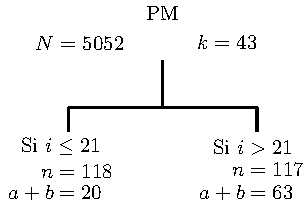
\includegraphics[width=4cm]{Graficos/e-figura1}
		
		%%
		%
		%	CAMBIAAAAAAAR
		%
		\caption{}
		\label{fig:e-figura1}
	\end{figure}
\end{observ}

\begin{observ}
	En el ejemplo \eqref{ejem-6.2}, el tamaño de la muestra obtenida con muestreo aleatorio simple es igual a \(115\), que por los ajustes necesarios en el muestreo sistemático aplicado, el tamaño de la muestra es igual a \(117\) o \(118\), dependiendo del elemento de inicio \(i\).
	
	Aparentemente, la diferencia en el tamaño de la muestra no es significativa; pero, en ciertos procesos es indispensable realizar esos ajustes para evitar que al final se pierda información de elementos que podrían representar cambios en la calidad de la producción. Por ejemplo, en la fabricación de piezas con maquinaria posible de recalentamiento o el tipo de materia prima utilizada.
\end{observ}

\begin{observ}
	Es conveniente presentar en la figura resumen, como la figura \eqref{fig:e-figura1}, el resultado de \(a+b\) dependiendo del valor de inicio \(i\) podría ser significativo para los interesados, tomar un elemento aleatorio adicional al principio o al final por cuestiones de calidad o un mejor conocimiento del comportamiento de los elementos de la población.
	
	
	En el ejemplo \eqref{ejem-6.2}.
	
	Si aleatoriamente se inicia en el elemento \(18\), \(a=17\) y \(b=3\). Podría ser de interés tomar aleatoriamente un elemento adicional entre los primeros 17 para analizar cómo comienza el proceso de producción o servicio.
	
	Si aleatoriamente se inicia en el elemento 25. \(a=24\) y \(b=39\). Podría ser de interés tomar aleatoriamente un elemento adicional entre los 39 últimos para analizar cómo culmina el proceso de producción o servicio.
	
	Eso se debe analizar considerando los costos o tiempo que representa incrementar adicionalmente
	un elemento en el proceso de muestreo sistemático.
\end{observ}


\begin{ejem}
	En un proceso de producción de 2236 unidades se conoce que la desviación estándar del proceso es igual a 6.4 libras. Obtenga el plan de muestreo sistemático si el límite para el error de estimación para la media del proceso es igual a 1.33 libras.
\end{ejem}
\begin{proof}[Solución]
		\(N=2236\); \(\sigma=6.4\); \(B=1.33\). No hay fija el nivel de confianza, se supone \(\gamma=0.95\),
		
		\(B=z_{\nicefrac{\alpha}{2}}\sqrt{\hat{\Var}[\bar{X}]}=\dfrac{\sigma^2}{n}\left(\dfrac{N-n}{N-1}\right)\); \(B=z_{\nicefrac{\alpha}{2}}\sqrt{\dfrac{\sigma^2(N-n)}{n(N-1)}}\); 
		
		\(P(Z<z_{\nicefrac{\alpha}{2}})=0.975\); \(z_{\nicefrac{\alpha}{2}}=1.96\);
		
		\(n=\dfrac{z_{\nicefrac{\alpha}{2}}\sigma^2N}{B^2(N-1)+z_{\nicefrac{\alpha}{2}}^2\sigma^2}=\dfrac{1.96^2 \times 6.4^2 \times 2236}{1.33^2 \times 2235+1.96^2 \times 6.4^2}=85.588\); \(n=86\)
		
		\(\dfrac{N}{n}=\dfrac{2236}{26}=26\); \(k=26\); \(e=0\); \(r=0\)
		
		No es posible incrementar una unidad en la muestra.
		
		Para comprobar lo obtenido: \(i=6\); \(a=5\); \(l=6+85 \times 26=2216\); \(b=2236-2216=20\); \(a+b=25\). No es posible incrementar una unidad en la muestra.
		
		PM: \(N=2236\); \(n=86\); \(k=26\)
\end{proof}

\begin{ejem}
	En la segunda parte del problema del ejemplo \eqref{ejem-5.7} se ha resuelto tomar la muestra sistemáticamente. Obtenga el plan de muestreo sistemático que garantice la participación de la mayor cantidad posible de elementos de la población.
\end{ejem}
\begin{proof}[Solución]\qquad
	
		\(N=365\); \(n=43\)
		
		\(\dfrac{N}{n}=\dfrac{365}{43}=8.488\); \(k=8\); \(e=0.488\); \(r=42 \times e=20.5116\)
		
		\(\left[\dfrac{r}{k}\right]=\left[\dfrac{20.5116}{8}\right]=[2.5639]=2\). De aproximadamente \(20\) elementos de la población se pueden tomar \(2\) de cada \(8\); por lo tanto \(n=45\).
		
		\(\dfrac{N}{n}=\dfrac{365}{45}=8.1111\); \(k=8\); \(e=0.1111\); \(r=44 \times e=4.888\)
		
		Como \(r=4.888<k=8\), se incrementa un elemento en la muestra hasta cierto \(i\).
		
		Tomando un elemento \(i\leq k\); por el ejemplo \(i=3\), \(a=2\);
		\(l=i+(n-1) \times k=3+44 \times 8=355\); \(b=N-l=365-355=10\); \(a+b=2+10=12\); se ratifica que se incrementa un elemento en la muestra hasta cierto \(i\).
		
		¿Hasta qué \(i\) se incrementa la muestra en una unidad?
		Hasta \(i=a+b-k+1=12-8+1=5\), o, \(i=N-nk=365-45 \times 8=5\)	\qedhere
		\begin{figure}[H]
			\centering
			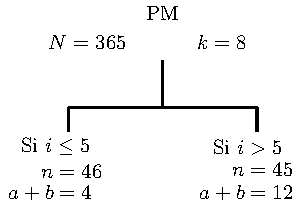
\includegraphics[width=4.5cm]{Graficos/e-figura2}
%			\caption{}
%			\label{fig:e-figura2}
		\end{figure}
		
\end{proof}


\begin{ejem}
	Por muestreo piloto anterior se conoce que el \(63\%\) de las \(4556\) personas están de acuerdo con la atención que reciben en el centro comercial donde realizan sus compras.
	
	Para realizar el estudio definitivo se ha fijado que el límite para el error de estimación para la proporción de personas que están de acuerdo con la atención que reciben sea igual al \(4.73\%\) y que el nivel de confianza sea igual al \(90\%\). Obtenga el plan de muestreo sistemático que garantice la participación de la mayor cantidad posible de elementos de la población.
\end{ejem}
\begin{proof}[Solución]
		\(N=4556\); \(\hat{p}=0.63\); \(B=0.473\); \(\gamma=0.90\); \(P(Z>z_{\nicefrac{\alpha}{2}})=0.95\); \(z_{\nicefrac{\alpha}{2}}=1.645\)
		
		\(B=z_{\nicefrac{\alpha}{2}}\sqrt{\hat{\Var}[\hat{P}]}\); \(\hat{\Var}[\hat{P}]=\dfrac{\hat{p}\hat{q}}{n-1}\left(\dfrac{N-n}{N}\right)\); \(B=z_{\nicefrac{\alpha}{2}}\sqrt{\dfrac{\hat{p}\hat{q}(N-n)}{(n-1)N}}\); \(n=\dfrac{z_{\nicefrac{\alpha}{2}}^2\hat{p}\hat{q} N+B^2N}{B^2N+z_{\nicefrac{\alpha}{2}}^2\hat{p}\hat{q}}\)
		
		\(n=\dfrac{1.645^2 \times 0.63 \times 0.37 \times 4556+0.0473^2 \times 4556}{0.0473^2 \times 4556+1.645^2 \times 0.63 \times 0.37}=266.448\); \(n=267\)
		
		\(\dfrac{N}{n}=\dfrac{4556}{267}=17.0636\); \(k=17\); \(e=0.0636\); \(r=266 \times e=16.936\)
		
		Como \(r=16.936<k=17\), se incrementa un elemento en la muestra hasta cierto \(i\).
		
		Tomando \(i=8\), \(a=7\); \(l=i+(n-1) \times k=8+266 \times 17=4530\); \(b=N-l=4556-4530=26\); \(a+b=7+26=33\); se ratifica que se incrementa un elemento en la muestra hasta cierto  \(i\).
		
		¿Hasta qué \(i\) se incrementa la muestra en una unidad?
		
		Hasta \(i=a+b-k+1=33-17+1=17\), o, \(i=N-nk=4556-267 \times 17=17\).
		
		Por lo tanto PM: \(N=4556\); \(n=268\); \(k=17\).
\end{proof}


\nocite{E-1, E-2, E-3, E-4, E-5}
}

\newpage
\newgeometry{top=2cm, bottom=2cm, left=1cm, right=1cm, headheight=1.8cm,headsep=.5cm,footskip=1.3cm}


\begin{table}[H]
\fontsize{6.5}{6.3}\selectfont
\captionsetup{justification=centering, labelfont=footnotesize, font=footnotesize}
  \centering
  \vspace{-4.5em}
  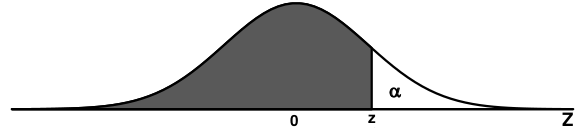
\includegraphics[width=0.55\linewidth]{Graficos/e-d-n}
%
	\[F(z)=P(Z\leq z)=\int_{-\infty}^{z}\dfrac{1}{\sqrt{2\pi}}e^{\nicefrac{t^2}{2}}=1-\alpha\]
    \begin{tabular}{c | cccccccccccc} \thickline
	$z$ & 0.00&0.01&0.02&0.03&0.04&0.05&0.06&0.07&0.08&0.09
    \\ \hline
	0.0&0.5000&0.5040&0.5080&0.5120&0.5160&0.5199&0.5239&0.5279&0.5319&0.5359    \\
	0.1&0.5398&0.5438&0.5478&0.5517&0.5557&0.5596&0.5636&0.5675&0.5714&0.5753	\\
	0.2&0.5793&0.5832&0.5871&0.5910&0.5948&0.5987&0.6026&0.6064&0.6103&0.6141	\\
	0.3&0.6179&0.6217&0.6255&0.6293&0.6331&0.6368&0.6406&0.6443&0.6480&0.6517	\\
	0.4&0.6554&0.6591&0.6628&0.6664&0.6700&0.6736&0.6772&0.6808&0.6844&0.6879	\\
	0.5&0.6915&0.6950&0.6985&0.7019&0.7054&0.7088&0.7123&0.7157&0.7190&0.7224	\\
	0.6&0.7257&0.7291&0.7324&0.7357&0.7389&0.7422&0.7454&0.7486&0.7517&0.7549	\\
	0.7&0.7580&0.7611&0.7642&0.7673&0.7703&0.7734&0.7764&0.7794&0.7823&0.7852	\\
	0.8&0.7881&0.7910&0.7939&0.7967&0.7995&0.8023&0.8051&0.8078&0.8106&0.8133	\\
	0.9&0.8159&0.8186&0.8212&0.8238&0.8264&0.8289&0.8315&0.8340&0.8365&0.8389	\\
	1.0&0.8413&0.8438&0.8461&0.8485&0.8508&0.8531&0.8554&0.8577&0.8599&0.8621	\\
	1.1&0.8643&0.8665&0.8686&0.8708&0.8729&0.8749&0.8770&0.8790&0.8810&0.8830	\\
	1.2&0.8849&0.8869&0.8888&0.8907&0.8925&0.8944&0.8962&0.8980&0.8997&0.9015	\\
	1.3&0.9032&0.9049&0.9066&0.9082&0.9099&0.9115&0.9131&0.9147&0.9162&0.9177	\\
	1.4&0.9192&0.9207&0.9222&0.9236&0.9251&0.9265&0.9279&0.9292&0.9306&0.9319	\\
	1.5&0.9332&0.9345&0.9357&0.9370&0.9382&0.9394&0.9406&0.9418&0.9429&0.9441	\\
	1.6&0.9452&0.9463&0.9474&0.9484&0.9495&0.9505&0.9515&0.9525&0.9535&0.9545	\\
	1.7&0.9554&0.9564&0.9573&0.9582&0.9591&0.9599&0.9608&0.9616&0.9625&0.9633	\\
	1.8&0.9641&0.9649&0.9656&0.9664&0.9671&0.9678&0.9686&0.9693&0.9699&0.9706	\\
	1.9&0.9713&0.9719&0.9726&0.9732&0.9738&0.9744&0.9750&0.9756&0.9761&0.9767	\\
	2.0&0.9772&0.9778&0.9783&0.9788&0.9793&0.9798&0.9803&0.9808&0.9812&0.9817	\\
	2.1&0.9821&0.9826&0.9830&0.9834&0.9838&0.9842&0.9846&0.9850&0.9854&0.9857	\\
	2.2&0.9861&0.9864&0.9868&0.9871&0.9875&0.9878&0.9881&0.9884&0.9887&0.9890	\\
	2.3&0.9893&0.9896&0.9898&0.9901&0.9904&0.9906&0.9909&0.9911&0.9913&0.9916	\\
	2.4&0.9918&0.9920&0.9922&0.9925&0.9927&0.9929&0.9931&0.9932&0.9934&0.9936	\\
	2.5&0.9938&0.9940&0.9941&0.9943&0.9945&0.9946&0.9948&0.9949&0.9951&0.9952	\\
	2.6&0.9953&0.9955&0.9956&0.9957&0.9959&0.9960&0.9961&0.9962&0.9963&0.9964	\\
	2.7&0.9965&0.9966&0.9967&0.9968&0.9969&0.9970&0.9971&0.9972&0.9973&0.9974	\\
	2.8&0.9974&0.9975&0.9976&0.9977&0.9977&0.9978&0.9979&0.9979&0.9980&0.9981	\\
	2.9&0.9981&0.9982&0.9982&0.9983&0.9984&0.9984&0.9985&0.9985&0.9986&0.9986	\\
	3.0&0.9987&0.9987&0.9987&0.9988&0.9988&0.9989&0.9989&0.9989&0.9990&0.9990	\\
	3.1&0.9990&0.9991&0.9991&0.9991&0.9992&0.9992&0.9992&0.9992&0.9993&0.9993	\\
	3.2&0.9993&0.9993&0.9994&0.9994&0.9994&0.9994&0.9994&0.9995&0.9995&0.9995	\\
	3.3&0.9995&0.9995&0.9995&0.9996&0.9996&0.9996&0.9996&0.9996&0.9996&0.9997	\\
	3.4&0.9997&0.9997&0.9997&0.9997&0.9997&0.9997&0.9997&0.9997&0.9997&0.9998	\\
	3.5&0.9998&0.9998&0.9998&0.9998&0.9998&0.9998&0.9998&0.9998&0.9998&0.9998	\\
	3.6&0.9998&0.9998&0.9999&0.9999&0.9999&0.9999&0.9999&0.9999&0.9999&0.9999	\\
	3.7&0.9999&0.9999&0.9999&0.9999&0.9999&0.9999&0.9999&0.9999&0.9999&0.9999	\\
	3.8&0.9999&0.9999&0.9999&0.9999&0.9999&0.9999&0.9999&0.9999&0.9999&0.9999	\\
	3.9&1.0000&1.0000&1.0000&1.0000&1.0000&1.0000&1.0000&1.0000&1.0000&1.0000\\	
    \thickline
    \end{tabular}
    \caption{Distribución Normal}
\end{table}

\newpage

	

\begin{table}[H]
\setlength{\tabcolsep}{1.5pt}
%\renewcommand{\arraystretch}{1}

\fontsize{6}{7}\selectfont
\captionsetup{justification=centering, labelfont=footnotesize, font=footnotesize}
  \centering
  \vspace{-2.5em}
  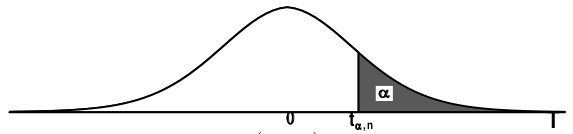
\includegraphics[width=0.55\linewidth]{Graficos/e-d-t}
%
	\[F(z)=P(T\geq t_{\alpha,n})=\alpha\]
    \begin{tabular}{c | ccccccccccccccccc} 
    \thickline
	\multirow{2}{*}{$\nu$} & \multicolumn{17}{c}{\(\alpha\)}
	\\
&0.200&0.150&0.100&0.090&0.080&0.070&0.060&0.050&0.045&0.040&0.035&0.030&0.025&0.020&0.015&0.010&0.005
    \\ \hline
	%
1&1.3764&1.9626&3.0777&3.4420&3.8947&4.4737&5.2422&6.3138&7.0264&7.9158&9.0579&10.579&12.706&15.895&21.205&31.821&63.657
\\
2&1.0607&1.3862&1.8856&2.0261&2.1894&2.3834&2.6202&2.9200&3.1040&3.3198&3.5782&3.8964&4.3027&4.8487&5.6428&6.9646&9.9248
\\
3&0.9785&1.2498&1.6377&1.7413&1.8589&1.9950&2.1562&2.3534&2.4708&2.6054&2.7626&2.9505&3.1824&3.4819&3.8960&4.5407&5.8409
\\
4&0.9410&1.1896&1.5332&1.6226&1.7229&1.8375&1.9712&2.1318&2.2261&2.3329&2.4559&2.6008&2.7764&2.9985&3.2976&3.7469&4.6041\\
5&0.9195&1.1558&1.4759&1.5579&1.6493&1.7529&1.8727&2.0150&2.0978&2.1910&2.2974&2.4216&2.5706&2.7565&3.0029&3.3649&4.0321\\
6&0.9057&1.1342&1.4398&1.5172&1.6033&1.7002&1.8117&1.9432&2.0192&2.1043&2.2011&2.3133&2.4469&2.6122&2.8289&3.1427&3.7074\\
7&0.8960&1.1192&1.4149&1.4894&1.5718&1.6643&1.7702&1.8946&1.9662&2.0460&2.1365&2.2409&2.3646&2.5168&2.7146&2.9980&3.4995\\
8&0.8889&1.1081&1.3968&1.4691&1.5489&1.6383&1.7402&1.8595&1.9280&2.0042&2.0902&2.1892&2.3060&2.4490&2.6338&2.8965&3.3554\\
9&0.8834&1.0997&1.3830&1.4537&1.5315&1.6185&1.7176&1.8331&1.8992&1.9727&2.0554&2.1504&2.2622&2.3984&2.5738&2.8214&3.2498\\
10&0.8791&1.0931&1.3722&1.4416&1.5179&1.6031&1.6998&1.8125&1.8768&1.9481&2.0283&2.1202&2.2281&2.3593&2.5275&2.7638&3.1693\\
11&0.8755&1.0877&1.3634&1.4318&1.5069&1.5906&1.6856&1.7959&1.8588&1.9284&2.0067&2.0961&2.2010&2.3281&2.4907&2.7181&3.1058\\
12&0.8726&1.0832&1.3562&1.4237&1.4979&1.5804&1.6739&1.7823&1.8440&1.9123&1.9889&2.0764&2.1788&2.3027&2.4607&2.6810&3.0545\\
13&0.8702&1.0795&1.3502&1.4170&1.4903&1.5718&1.6641&1.7709&1.8317&1.8989&1.9742&2.0600&2.1604&2.2816&2.4358&2.6503&3.0123\\
14&
0.8681&
1.0763&
1.3450&
1.4113&
1.4839&
1.5646&
1.6558&
1.7613&
1.8213&
1.8875&
1.9617&
2.0462&
2.1448&
2.2638&
2.4149&
2.6245&
2.9768\\
15&
0.8662&
1.0735&
1.3406&
1.4063&
1.4784&
1.5583&
1.6487&
1.7531&
1.8123&
1.8777&
1.9509&
2.0343&
2.1314&
2.2485&
2.3970&
2.6025&
2.9467\\
16&
0.8647&
1.0711&
1.3368&
1.4021&
1.4736&
1.5529&
1.6425&
1.7459&
1.8046&
1.8693&
1.9417&
2.0240&
2.1199&
2.2354&
2.3815&
2.5835&
2.9208\\
17&
0.8633&
1.0690&
1.3334&
1.3983&
1.4694&
1.5482&
1.6370&
1.7396&
1.7978&
1.8619&
1.9335&
2.0150&
2.1098&
2.2238&
2.3681&
2.5669&
2.8982\\
18&
0.8620&
1.0672&
1.3304&
1.3950&
1.4656&
1.5439&
1.6322&
1.7341&
1.7918&
1.8553&
1.9264&
2.0071&
2.1009&
2.2137&
2.3562&
2.5524&
2.8784\\
19&
0.8610&
1.0655&
1.3277&
1.3920&
1.4623&
1.5402&
1.6280&
1.7291&
1.7864&
1.8495&
1.9200&
2.0000&
2.0930&
2.2047&
2.3456&
2.5395&
2.8609\\
20&
0.8600&
1.0640&
1.3253&
1.3894&
1.4593&
1.5369&
1.6242&
1.7247&
1.7816&
1.8443&
1.9143&
1.9937&
2.0860&
2.1967&
2.3362&
2.5280&
2.8453\\
21&
0.8591&
1.0627&
1.3232&
1.3870&
1.4567&
1.5338&
1.6207&
1.7207&
1.7773&
1.8397&
1.9092&
1.9880&
2.0796&
2.1894&
2.3278&
2.5176&
2.8314\\
22&
0.8583&
1.0614&
1.3212&
1.3848&
1.4542&
1.5311&
1.6176&
1.7171&
1.7734&
1.8354&
1.9045&
1.9829&
2.0739&
2.1829&
2.3202&
2.5083&
2.8188\\
23&
0.8575&
1.0603&
1.3195&
1.3828&
1.4520&
1.5286&
1.6148&
1.7139&
1.7699&
1.8316&
1.9003&
1.9782&
2.0687&
2.1770&
2.3132&
2.4999&
2.8073\\
24&
0.8569&
1.0593&
1.3178&
1.3810&
1.4500&
1.5263&
1.6122&
1.7109&
1.7667&
1.8281&
1.8965&
1.9740&
2.0639&
2.1715&
2.3069&
2.4922&
2.7969\\
25&
0.8562&
1.0584&
1.3163&
1.3794&
1.4482&
1.5242&
1.6098&
1.7081&
1.7637&
1.8248&
1.8929&
1.9701&
2.0595&
2.1666&
2.3011&
2.4851&
2.7874\\
26&
0.8557&
1.0575&
1.3150&
1.3778&
1.4464&
1.5223&
1.6076&
1.7056&
1.7610&
1.8219&
1.8897&
1.9665&
2.0555&
2.1620&
2.2958&
2.4786&
2.7787\\
27&
0.8551&
1.0567&
1.3137&
1.3764&
1.4449&
1.5205&
1.6056&
1.7033&
1.7585&
1.8191&
1.8867&
1.9632&
2.0518&
2.1578&
2.2909&
2.4727&
2.7707\\
28&
0.8546&
1.0560&
1.3125&
1.3751&
1.4434&
1.5189&
1.6037&
1.7011&
1.7561&
1.8166&
1.8839&
1.9601&
2.0484&
2.1539&
2.2864&
2.4671&
2.7633\\
29&
0.8542&
1.0553&
1.3114&
1.3739&
1.4421&
1.5174&
1.6020&
1.6991&
1.7540&
1.8142&
1.8813&
1.9573&
2.0452&
2.1503&
2.2822&
2.4620&
2.7564\\
30&
0.8538&
1.0547&
1.3104&
1.3728&
1.4408&
1.5159&
1.6004&
1.6973&
1.7520&
1.8120&
1.8789&
1.9546&
2.0423&
2.1470&
2.2783&
2.4573&
2.7500\\
35&
0.8520&
1.0520&
1.3062&
1.3681&
1.4356&
1.5101&
1.5937&
1.6896&
1.7436&
1.8030&
1.8691&
1.9438&
2.0301&
2.1332&
2.2622&
2.4377&
2.7238\\
40&
0.8507&
1.0500&
1.3031&
1.3646&
1.4317&
1.5057&
1.5887&
1.6839&
1.7375&
1.7963&
1.8617&
1.9357&
2.0211&
2.1229&
2.2503&
2.4233&
2.7045\\
45&
0.8497&
1.0485&
1.3006&
1.3619&
1.4287&
1.5023&
1.5849&
1.6794&
1.7327&
1.7911&
1.8561&
1.9294&
2.0141&
2.1150&
2.2411&
2.4121&
2.6896\\
50&
0.8489&
1.0473&
1.2987&
1.3598&
1.4263&
1.4996&
1.5818&
1.6759&
1.7289&
1.7870&
1.8516&
1.9244&
2.0086&
2.1087&
2.2338&
2.4033&
2.6778\\
55&
0.8482&
1.0463&
1.2971&
1.3580&
1.4243&
1.4974&
1.5793&
1.6730&
1.7258&
1.7836&
1.8479&
1.9204&
2.0040&
2.1036&
2.2278&
2.3961&
2.6682\\
60&
0.8477&
1.0455&
1.2958&
1.3566&
1.4227&
1.4956&
1.5772&
1.6706&
1.7232&
1.7808&
1.8448&
1.9170&
2.0003&
2.0994&
2.2229&
2.3901&
2.6603\\
65&
0.8472&
1.0448&
1.2947&
1.3553&
1.4213&
1.4941&
1.5755&
1.6686&
1.7210&
1.7785&
1.8423&
1.9142&
1.9971&
2.0958&
2.2188&
2.3851&
2.6536\\
70&
0.8468&
1.0442&
1.2938&
1.3543&
1.4202&
1.4927&
1.5740&
1.6669&
1.7192&
1.7765&
1.8401&
1.9118&
1.9944&
2.0927&
2.2152&
2.3808&
2.6479\\
75&
0.8464&
1.0436&
1.2929&
1.3534&
1.4191&
1.4916&
1.5727&
1.6654&
1.7176&
1.7747&
1.8381&
1.9097&
1.9921&
2.0901&
2.2122&
2.3771&
2.6430\\
80&
0.8461&
1.0432&
1.2922&
1.3526&
1.4183&
1.4906&
1.5716&
1.6641&
1.7162&
1.7732&
1.8365&
1.9078&
1.9901&
2.0878&
2.2095&
2.3739&
2.6387
\\
    \thickline
    \end{tabular}
    \caption{Distribución \(t\) de Student -- (a)}
\end{table}	
	
\begin{table}[H]
\setlength{\tabcolsep}{1.5pt}
%\renewcommand{\arraystretch}{1}

\fontsize{6}{7}\selectfont
\captionsetup{justification=centering, labelfont=footnotesize, font=footnotesize}
  \centering
  \vspace{-2.5em}
  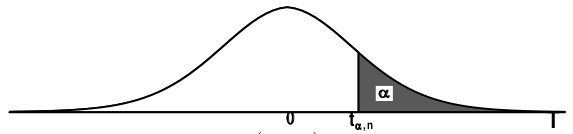
\includegraphics[width=0.55\linewidth]{Graficos/e-d-t}
%
	\[F(z)=P(T\geq t_{\alpha,n})=\alpha\]
    \begin{tabular}{c | ccccccccccccccccc} 
    \thickline
	\multirow{2}{*}{$\nu$} & \multicolumn{17}{c}{\(\alpha\)}
	\\
&0.200&0.150&0.100&0.090&0.080&0.070&0.060&0.050&0.045&0.040&0.035&0.030&0.025&0.020&0.015&0.010&0.005
    \\ \hline
	%
85&
0.8459&
1.0428&
1.2916&
1.3519&
1.4175&
1.4897&
1.5706&
1.6630&
1.7149&
1.7719&
1.8350&
1.9062&
1.9883&
2.0857&
2.2071&
2.3710&
2.6349\\
90&
0.8456&
1.0424&
1.2910&
1.3513&
1.4168&
1.4889&
1.5697&
1.6620&
1.7138&
1.7707&
1.8337&
1.9048&
1.9867&
2.0839&
2.2050&
2.3685&
2.6316\\
95&
0.8454&
1.0421&
1.2905&
1.3507&
1.4162&
1.4882&
1.5689&
1.6611&
1.7129&
1.7696&
1.8326&
1.9035&
1.9853&
2.0823&
2.2032&
2.3662&
2.6286\\
100&
0.8452&
1.0418&
1.2901&
1.3502&
1.4156&
1.4876&
1.5682&
1.6602&
1.7120&
1.7687&
1.8315&
1.9024&
1.9840&
2.0809&
2.2015&
2.3642&
2.6259\\
105&
0.8451&
1.0416&
1.2897&
1.3497&
1.4151&
1.4870&
1.5675&
1.6595&
1.7112&
1.7678&
1.8306&
1.9013&
1.9828&
2.0796&
2.2000&
2.3624&
2.6235\\
110&
0.8449&
1.0413&
1.2893&
1.3493&
1.4146&
1.4865&
1.5669&
1.6588&
1.7105&
1.7670&
1.8297&
1.9004&
1.9818&
2.0784&
2.1986&
2.3607&
2.6213\\
115&
0.8448&
1.0411&
1.2890&
1.3490&
1.4142&
1.4861&
1.5664&
1.6582&
1.7098&
1.7663&
1.8289&
1.8995&
1.9808&
2.0773&
2.1974&
2.3592&
2.6193\\
120&
0.8446&
1.0409&
1.2886&
1.3486&
1.4138&
1.4856&
1.5659&
1.6577&
1.7092&
1.7656&
1.8282&
1.8987&
1.9799&
2.0763&
2.1962&
2.3578&
2.6174\\
125&
0.8445&
1.0408&
1.2884&
1.3483&
1.4135&
1.4852&
1.5655&
1.6571&
1.7086&
1.7650&
1.8276&
1.8980&
1.9791&
2.0754&
2.1951&
2.3565&
2.6157\\
130&
0.8444&
1.0406&
1.2881&
1.3480&
1.4132&
1.4849&
1.5651&
1.6567&
1.7081&
1.7645&
1.8270&
1.8973&
1.9784&
2.0746&
2.1942&
2.3554&
2.6142\\
135&
0.8443&
1.0404&
1.2879&
1.3477&
1.4129&
1.4845&
1.5647&
1.6562&
1.7076&
1.7640&
1.8264&
1.8967&
1.9777&
2.0738&
2.1933&
2.3543&
2.6127\\
140&
0.8442&
1.0403&
1.2876&
1.3475&
1.4126&
1.4842&
1.5643&
1.6558&
1.7072&
1.7635&
1.8259&
1.8962&
1.9771&
2.0731&
2.1924&
2.3533&
2.6114\\
145&
0.8441&
1.0402&
1.2874&
1.3473&
1.4123&
1.4839&
1.5640&
1.6554&
1.7068&
1.7630&
1.8254&
1.8956&
1.9765&
2.0724&
2.1917&
2.3523&
2.6102\\
150&
0.8440&
1.0400&
1.2872&
1.3470&
1.4121&
1.4836&
1.5637&
1.6551&
1.7064&
1.7626&
1.8249&
1.8951&
1.9759&
2.0718&
2.1909&
2.3515&
2.6090\\
169&
0.8438&
1.0396&
1.2866&
1.3463&
1.4113&
1.4828&
1.5627&
1.6539&
1.7052&
1.7613&
1.8235&
1.8935&
1.9741&
2.0697&
2.1886&
2.3486&
2.6052\\
188&
0.8435&
1.0393&
1.2861&
1.3458&
1.4107&
1.4821&
1.5619&
1.6530&
1.7042&
1.7602&
1.8223&
1.8922&
1.9727&
2.0681&
2.1867&
2.3463&
2.6022\\
207&
0.8434&
1.0390&
1.2857&
1.3453&
1.4101&
1.4815&
1.5612&
1.6522&
1.7034&
1.7593&
1.8213&
1.8912&
1.9715&
2.0668&
2.1852&
2.3445&
2.5998\\
226&
0.8432&
1.0388&
1.2853&
1.3449&
1.4097&
1.4810&
1.5607&
1.6516&
1.7027&
1.7586&
1.8205&
1.8903&
1.9705&
2.0657&
2.1839&
2.3430&
2.5978\\
245&
0.8431&
1.0386&
1.2850&
1.3446&
1.4093&
1.4806&
1.5602&
1.6511&
1.7021&
1.7580&
1.8199&
1.8895&
1.9697&
2.0647&
2.1828&
2.3417&
2.5960\\
264&
0.8430&
1.0385&
1.2848&
1.3443&
1.4090&
1.4802&
1.5598&
1.6506&
1.7016&
1.7575&
1.8193&
1.8889&
1.9690&
2.0639&
2.1819&
2.3406&
2.5946\\
283&
0.8429&
1.0383&
1.2846&
1.3441&
1.4088&
1.4799&
1.5595&
1.6503&
1.7012&
1.7570&
1.8188&
1.8884&
1.9684&
2.0633&
2.1811&
2.3396&
2.5933\\
302&
0.8428&
1.0382&
1.2844&
1.3439&
1.4085&
1.4797&
1.5592&
1.6499&
1.7009&
1.7566&
1.8184&
1.8879&
1.9679&
2.0627&
2.1804&
2.3388&
2.5922\\
401&
0.8425&
1.0378&
1.2837&
1.3431&
1.4077&
1.4787&
1.5581&
1.6487&
1.6995&
1.7551&
1.8168&
1.8861&
1.9659&
2.0605&
2.1778&
2.3357&
2.5881\\
500&
0.8423&
1.0375&
1.2832&
1.3426&
1.4072&
1.4781&
1.5574&
1.6479&
1.6987&
1.7543&
1.8158&
1.8851&
1.9647&
2.0591&
2.1763&
2.3338&
2.5857\\
599&
0.8422&
1.0373&
1.2830&
1.3423&
1.4068&
1.4778&
1.5570&
1.6474&
1.6981&
1.7537&
1.8152&
1.8844&
1.9639&
2.0582&
2.1753&
2.3326&
2.5841\\
\(\infty\)&
0.8416&
1.0364&
1.2816&
1.3408&
1.4051&
1.4758&
1.5548&
1.6449&
1.6954&
1.7507&
1.8119&
1.8808&
1.9600&
2.0538&
2.1701&
2.3264&
2.5758
\\
    \thickline
    \end{tabular}
    \caption{Distribución \(t\) de Student -- (b)}
\end{table}		
	
	
	

%
%
%
%
%
%
%
%
%
%
%
%
%
%
%
%
%
%
%
%
%
%
%
%
%
%
%
%
%
%
%
%
%
%

%\vfill
%\newpage
%\newgeometry{top=2cm, bottom=2cm, left=2cm, right=2cm, headheight=1.8cm,headsep=.5cm,footskip=1.3cm}






\end{document}































